% Options for packages loaded elsewhere
\PassOptionsToPackage{unicode}{hyperref}
\PassOptionsToPackage{hyphens}{url}
%
\documentclass[
]{article}
\usepackage{lmodern}
\usepackage{amssymb,amsmath}
\usepackage{ifxetex,ifluatex}
\ifnum 0\ifxetex 1\fi\ifluatex 1\fi=0 % if pdftex
  \usepackage[T1]{fontenc}
  \usepackage[utf8]{inputenc}
  \usepackage{textcomp} % provide euro and other symbols
\else % if luatex or xetex
  \usepackage{unicode-math}
  \defaultfontfeatures{Scale=MatchLowercase}
  \defaultfontfeatures[\rmfamily]{Ligatures=TeX,Scale=1}
\fi
% Use upquote if available, for straight quotes in verbatim environments
\IfFileExists{upquote.sty}{\usepackage{upquote}}{}
\IfFileExists{microtype.sty}{% use microtype if available
  \usepackage[]{microtype}
  \UseMicrotypeSet[protrusion]{basicmath} % disable protrusion for tt fonts
}{}
\makeatletter
\@ifundefined{KOMAClassName}{% if non-KOMA class
  \IfFileExists{parskip.sty}{%
    \usepackage{parskip}
  }{% else
    \setlength{\parindent}{0pt}
    \setlength{\parskip}{6pt plus 2pt minus 1pt}}
}{% if KOMA class
  \KOMAoptions{parskip=half}}
\makeatother
\usepackage{xcolor}
\IfFileExists{xurl.sty}{\usepackage{xurl}}{} % add URL line breaks if available
\IfFileExists{bookmark.sty}{\usepackage{bookmark}}{\usepackage{hyperref}}
\hypersetup{
  hidelinks,
  pdfcreator={LaTeX via pandoc}}
\urlstyle{same} % disable monospaced font for URLs
\usepackage{longtable,booktabs}
% Correct order of tables after \paragraph or \subparagraph
\usepackage{etoolbox}
\makeatletter
\patchcmd\longtable{\par}{\if@noskipsec\mbox{}\fi\par}{}{}
\makeatother
% Allow footnotes in longtable head/foot
\IfFileExists{footnotehyper.sty}{\usepackage{footnotehyper}}{\usepackage{footnote}}
\makesavenoteenv{longtable}
\usepackage{graphicx}
\makeatletter
\def\maxwidth{\ifdim\Gin@nat@width>\linewidth\linewidth\else\Gin@nat@width\fi}
\def\maxheight{\ifdim\Gin@nat@height>\textheight\textheight\else\Gin@nat@height\fi}
\makeatother
% Scale images if necessary, so that they will not overflow the page
% margins by default, and it is still possible to overwrite the defaults
% using explicit options in \includegraphics[width, height, ...]{}
\setkeys{Gin}{width=\maxwidth,height=\maxheight,keepaspectratio}
% Set default figure placement to htbp
\makeatletter
\def\fps@figure{htbp}
\makeatother
\setlength{\emergencystretch}{3em} % prevent overfull lines
\providecommand{\tightlist}{%
  \setlength{\itemsep}{0pt}\setlength{\parskip}{0pt}}
\setcounter{secnumdepth}{-\maxdimen} % remove section numbering

\author{Jakub Dokulil}
\date{2021}

\usepackage[czech]{babel}

\begin{document}


\hypertarget{projekt-dalekohledu-pro-pux159edmux11bt-tkc}{%
\section{Projekt dalekohledu pro předmět
TKC}\label{projekt-dalekohledu-pro-pux159edmux11bt-tkc}}

Jakub Dokulil, 2021

\begin{figure}
\centering

\includegraphics{imgs/dalekohledy_1.png}
\caption{Dalekohledy}
\end{figure}

\section*{Úvod}
Cílem tohoto projektu je navrhnout dalekohled keplerova uspočádání. Čili dalekohled se bude skládat z objektivu a okuláru s určením pro pozemní pozorování. Jako převracecí mechanismus bude použito zrcátko. Inspiraci jsem si vzal z dalekohledu od společnosti \href{https://eshop.meopta.cz/spektivy/}{Meopta}.

\hypertarget{rozvrux17eenuxed}{%
\subsection{Rozvržení}\label{rozvrux17eenuxed}}

Konstrukce je inspirována spektivem
\href{https://eshop.meopta.cz/spektivy-meostar-s2/spektiv-meostar-s2-82-hd-sikmy/}{Meopta
MeoStar S2} tento spektiv má ohniskovou vzdálenost objektivu 439 mm.

\begin{figure}
\centering
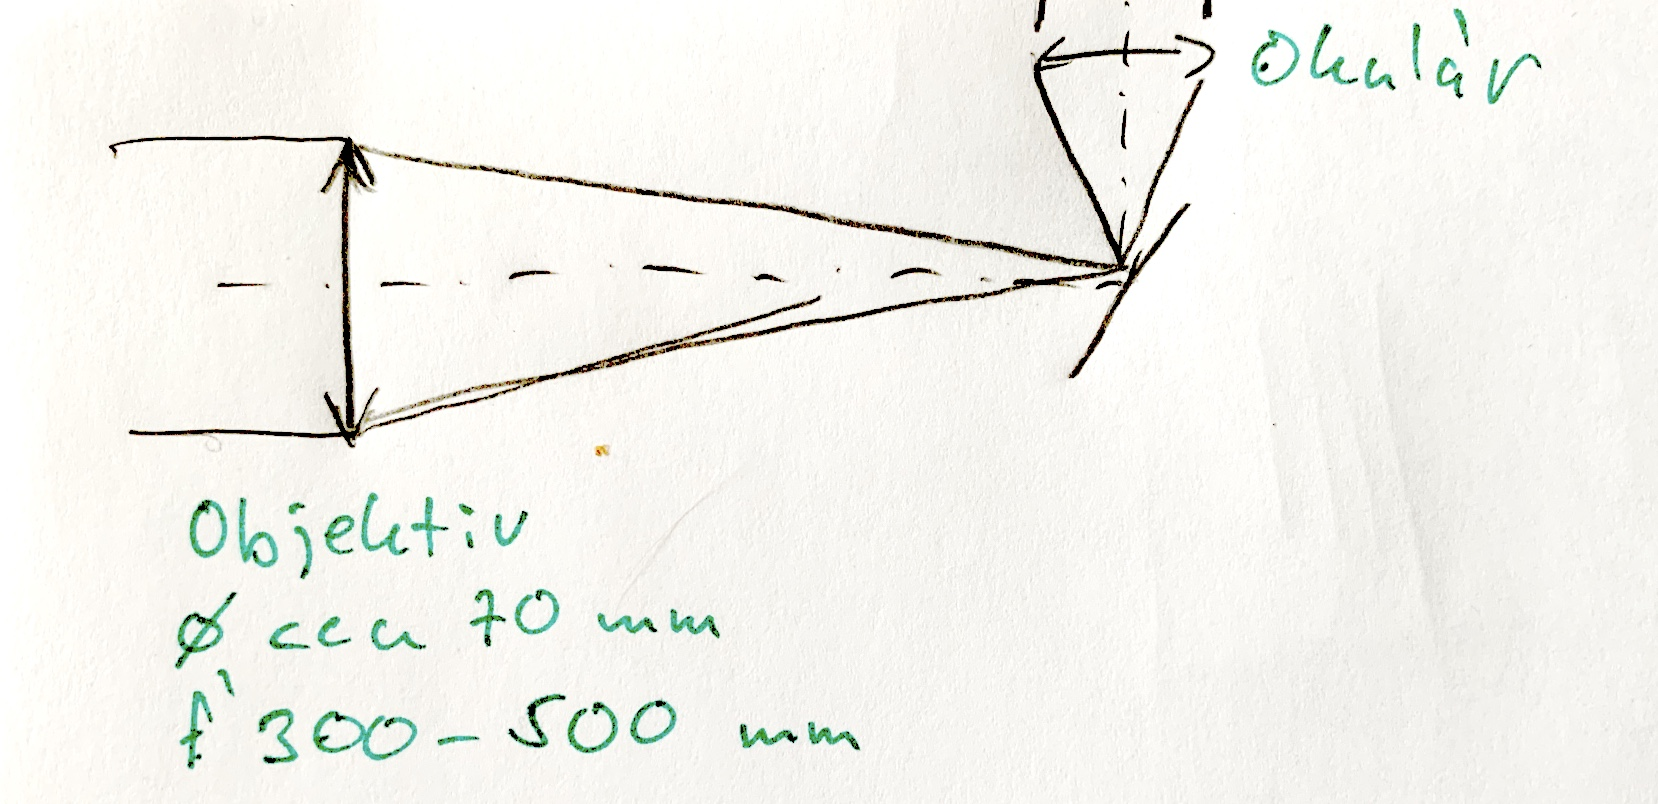
\includegraphics{imgs/rozvrzeni.jpeg}
\caption{rozvrzeni dalekohledu}
\end{figure}

Jako objektiv bude sloužit achromatický dublet. Například firma Edmund
Optics
\href{https://www.edmundoptics.com/c/achromatic-lenses/652/\#29374=29374_s\%3ANS4wMCAtIDUuOTk1\&29374=29374_s\%3ANC4wMCAtIDQuOTk1\&27560=27560_s\%3AVklTIDAmZGVnOyAoNDI1LTY3NW5tKQ2\&27560=27560_s\%3AVklTLU5JUiAoNDAwLTEwMDBubSk1\&27560=27560_s\%3ATWdGPHN1Yj4yPC9zdWI-ICg0MDAtNzAwbm0p0\&27560=27560_s\%3ATWdGPHN1Yj4yPC9zdWI-ICg0MDAtNzAwbm0p0\&27560=27560_s\%3AVklTIDAmZGVnOyAoNDI1LTY3NW5tKQ2\&27560=27560_s\%3AVklTLU5JUiAoNDAwLTEwMDBubSk1\&27560=27560_s\%3AVVYtVklTICgzNDUtNzAwbm0p0\&27614=27614_d\%3A\%5B59.18\%20TO\%2089.47\%5D}{nabízí}
takové dublety, které vyhovují průměrem ohniskem. Další výhodou je
knihovna dílů v programu Zemax Optics Studio.

Jako okulár se jeví vhodné použít
\href{https://eshop.meopta.cz/spektivy-meostar-s1/okular-20-60x/}{okulár
20-60x od společnosti Meopta}, navíc spektiv MeoStar S1 má ohniskovou
vzdálenost objektivu podobnou námi zvlené vzdálenosti (f' = 329 mm).
Díky tomu, že okulár umožňuje zoomovat není zapotřebí měnit okuláry, což
umožní redukovat množství prachu, které si při výměně do tubusu dostane.

\hypertarget{vuxfdbux11br-komponent-a-simulace-v-programu-zemax}{%
\subsection{Výběr komponent a simulace v programu
Zemax}\label{vuxfdbux11br-komponent-a-simulace-v-programu-zemax}}

\hypertarget{objektiv}{%
\subsubsection{Objektiv}\label{objektiv}}

Z nabídky
\href{https://www.edmundoptics.com/c/achromatic-lenses/652/\#29374=29374_s\%3ANS4wMCAtIDUuOTk1\&29374=29374_s\%3ANC4wMCAtIDQuOTk1\&27560=27560_s\%3AVklTIDAmZGVnOyAoNDI1LTY3NW5tKQ2\&27560=27560_s\%3AVklTLU5JUiAoNDAwLTEwMDBubSk1\&27560=27560_s\%3ATWdGPHN1Yj4yPC9zdWI-ICg0MDAtNzAwbm0p0\&27560=27560_s\%3ATWdGPHN1Yj4yPC9zdWI-ICg0MDAtNzAwbm0p0\&27560=27560_s\%3AVklTIDAmZGVnOyAoNDI1LTY3NW5tKQ2\&27560=27560_s\%3AVklTLU5JUiAoNDAwLTEwMDBubSk1\&27560=27560_s\%3AVVYtVklTICgzNDUtNzAwbm0p0\&27614=27614_d\%3A\%5B59.18\%20TO\%2089.47\%5D}{vhodných
achromatických dubletů}) firmy Edumnd Optics byl vybrát
\href{https://www.edmundoptics.com/p/75mm-dia-x-400mm-fl-vis-0deg-coated-achromatic-lens/30848/}{dublet}
s ohniskovou vzdáleností 400 mm a průměru 75 mm s vrstvou propouštející
viditelné vlnové délky (400 - 700 nm).

Jelikož je dalekohled určen pro pozemní pozorování, tak je zapotřebí
použít jako kameru vhodný fotoaparát. Samotný dublet nemusí mít velké
zorné pole, proto stačí použít fotoaparát s čipem micro 4/3, například
\href{https://www.fotoskoda.cz/panasonic-lumix-dc-gh5s/}{Panasonic Lumix
GHS5}. Rozměry čipu 17,3 na 13 mm znemenají, že nejvzdálenější objekt od
osy bude 10,8 mm.

Při simulaci je zapotřebí počítat se závitovým kroužkem upínajícím
objektiv do objímky, proto byla zvolena apertura o průměru 73 mm. Při
simulaci bylo simulováno zobrazení osového předmětu a dále předmětů
vzdálených 1° a 1,5° od osy pro pokrytí celého čipu.

\begin{figure}
\centering
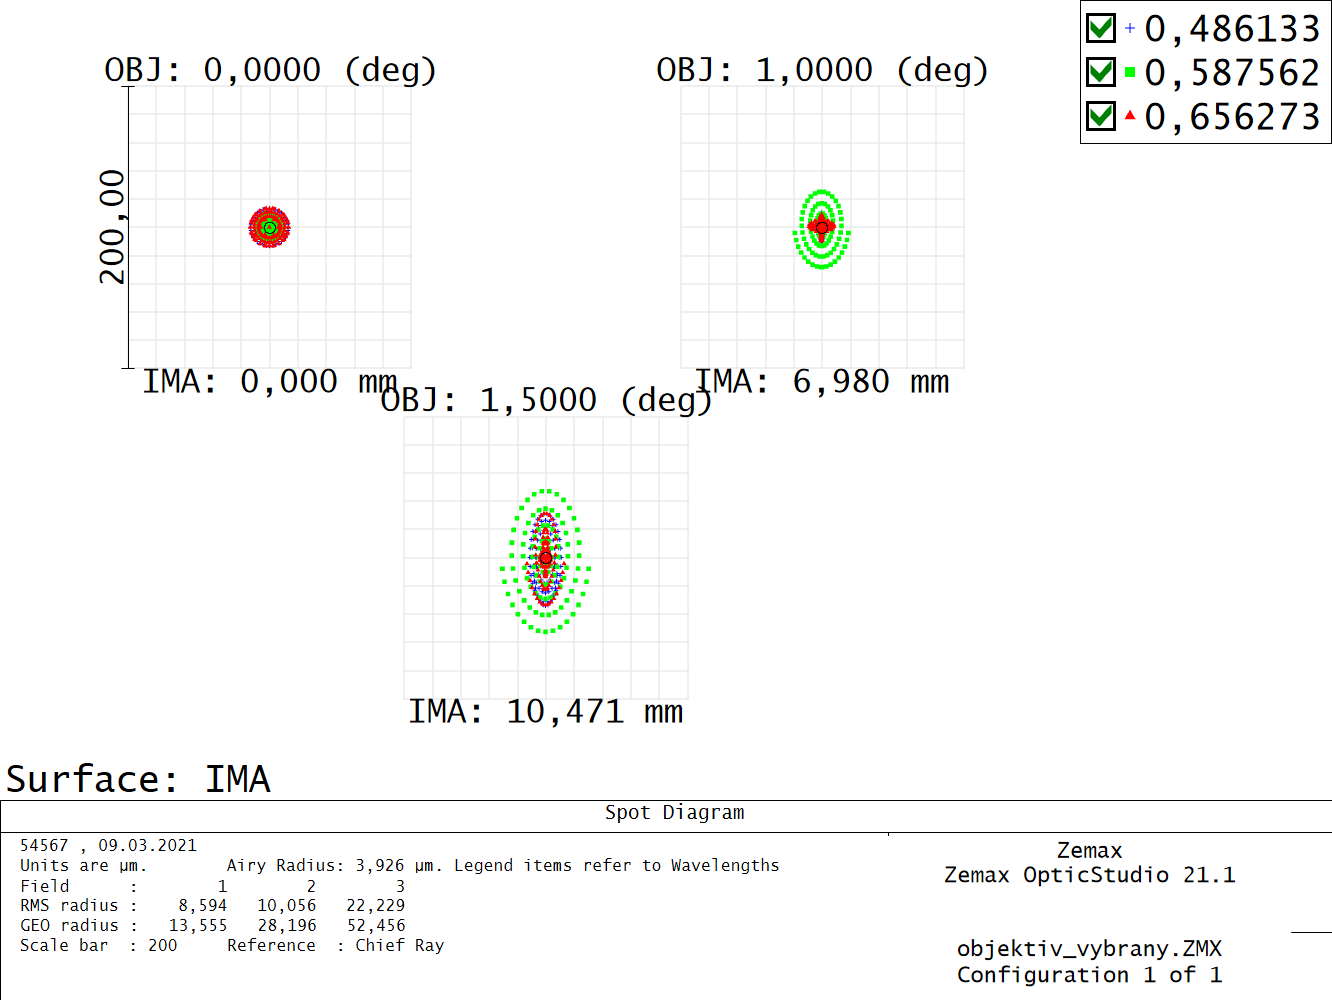
\includegraphics{imgs/SpotDiagram_dublet.png}
\caption{spot dubletu}
\end{figure}

Ze spot diagramu lze vidět, že pokud chceme získat kvalitní obraz
předmětu umístěného uprostřed zorného pole stačí velikost pixelu okolo
10 μm. To lze ostatně taktéž vidět na závislosti funkce přenosu
kontrastu (MTF - Modulated Transfer Funkction) na zorném poli. O clonách
pro odstínění parazitních paprsků bude pojednáno později.

\begin{figure}
\centering
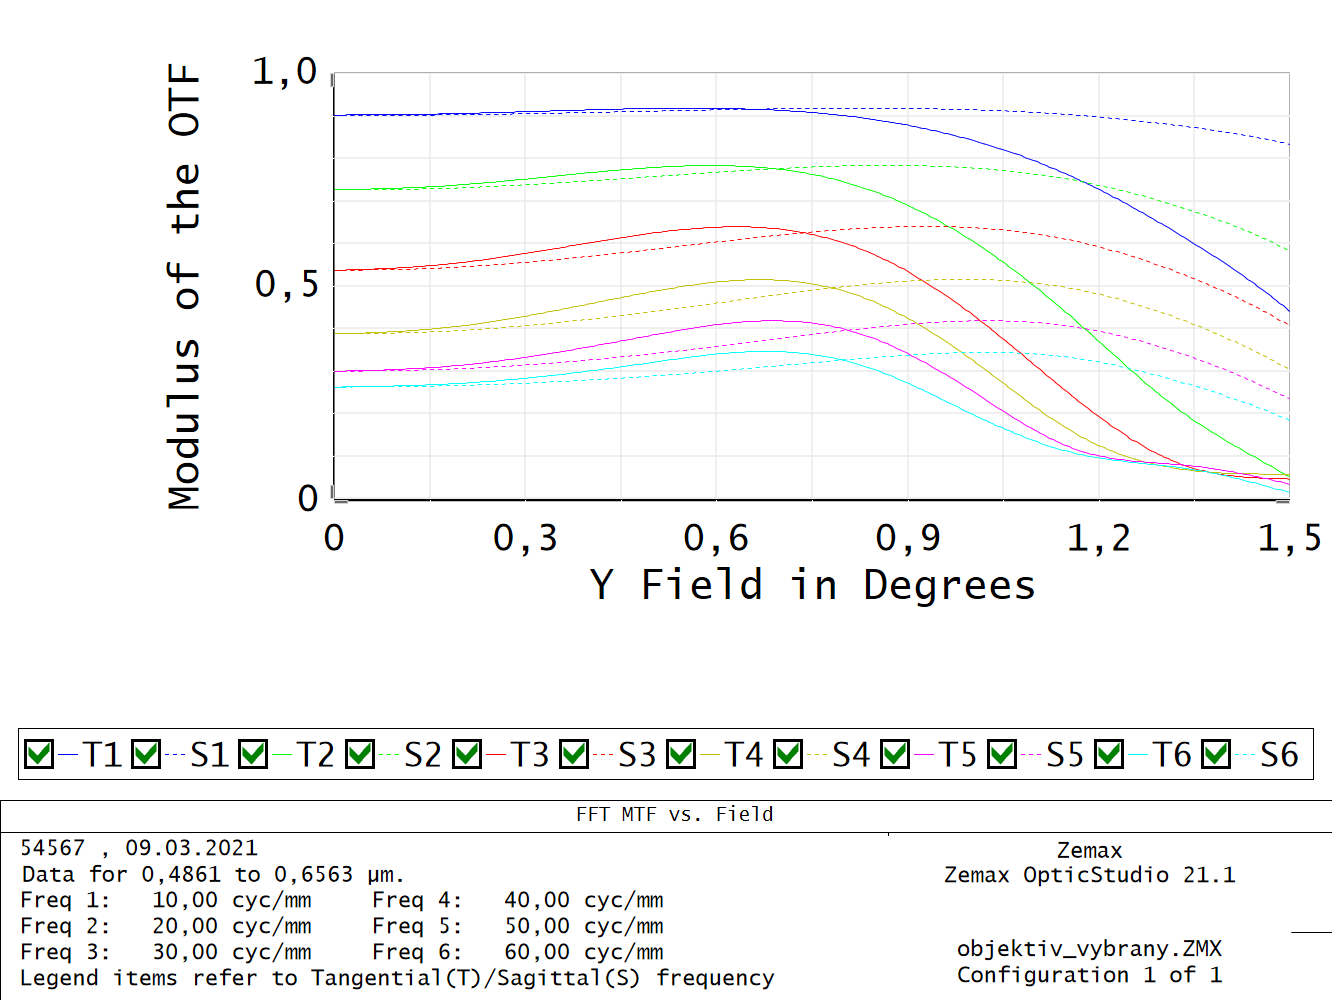
\includegraphics{imgs/FFTMTFvsField_dublet.png}
\caption{MTF}
\end{figure}

\hypertarget{okuluxe1r-a-pozorovuxe1nuxed-okem.}{%
\subsubsection{Okulár a pozorování
okem.}\label{okuluxe1r-a-pozorovuxe1nuxed-okem.}}

Při pozorování okem poskytuje samotný objektiv zorné pola max 2,4° Při
použití většího zorného pole, je zklenutí pole větší jak podélná
sférická vada.

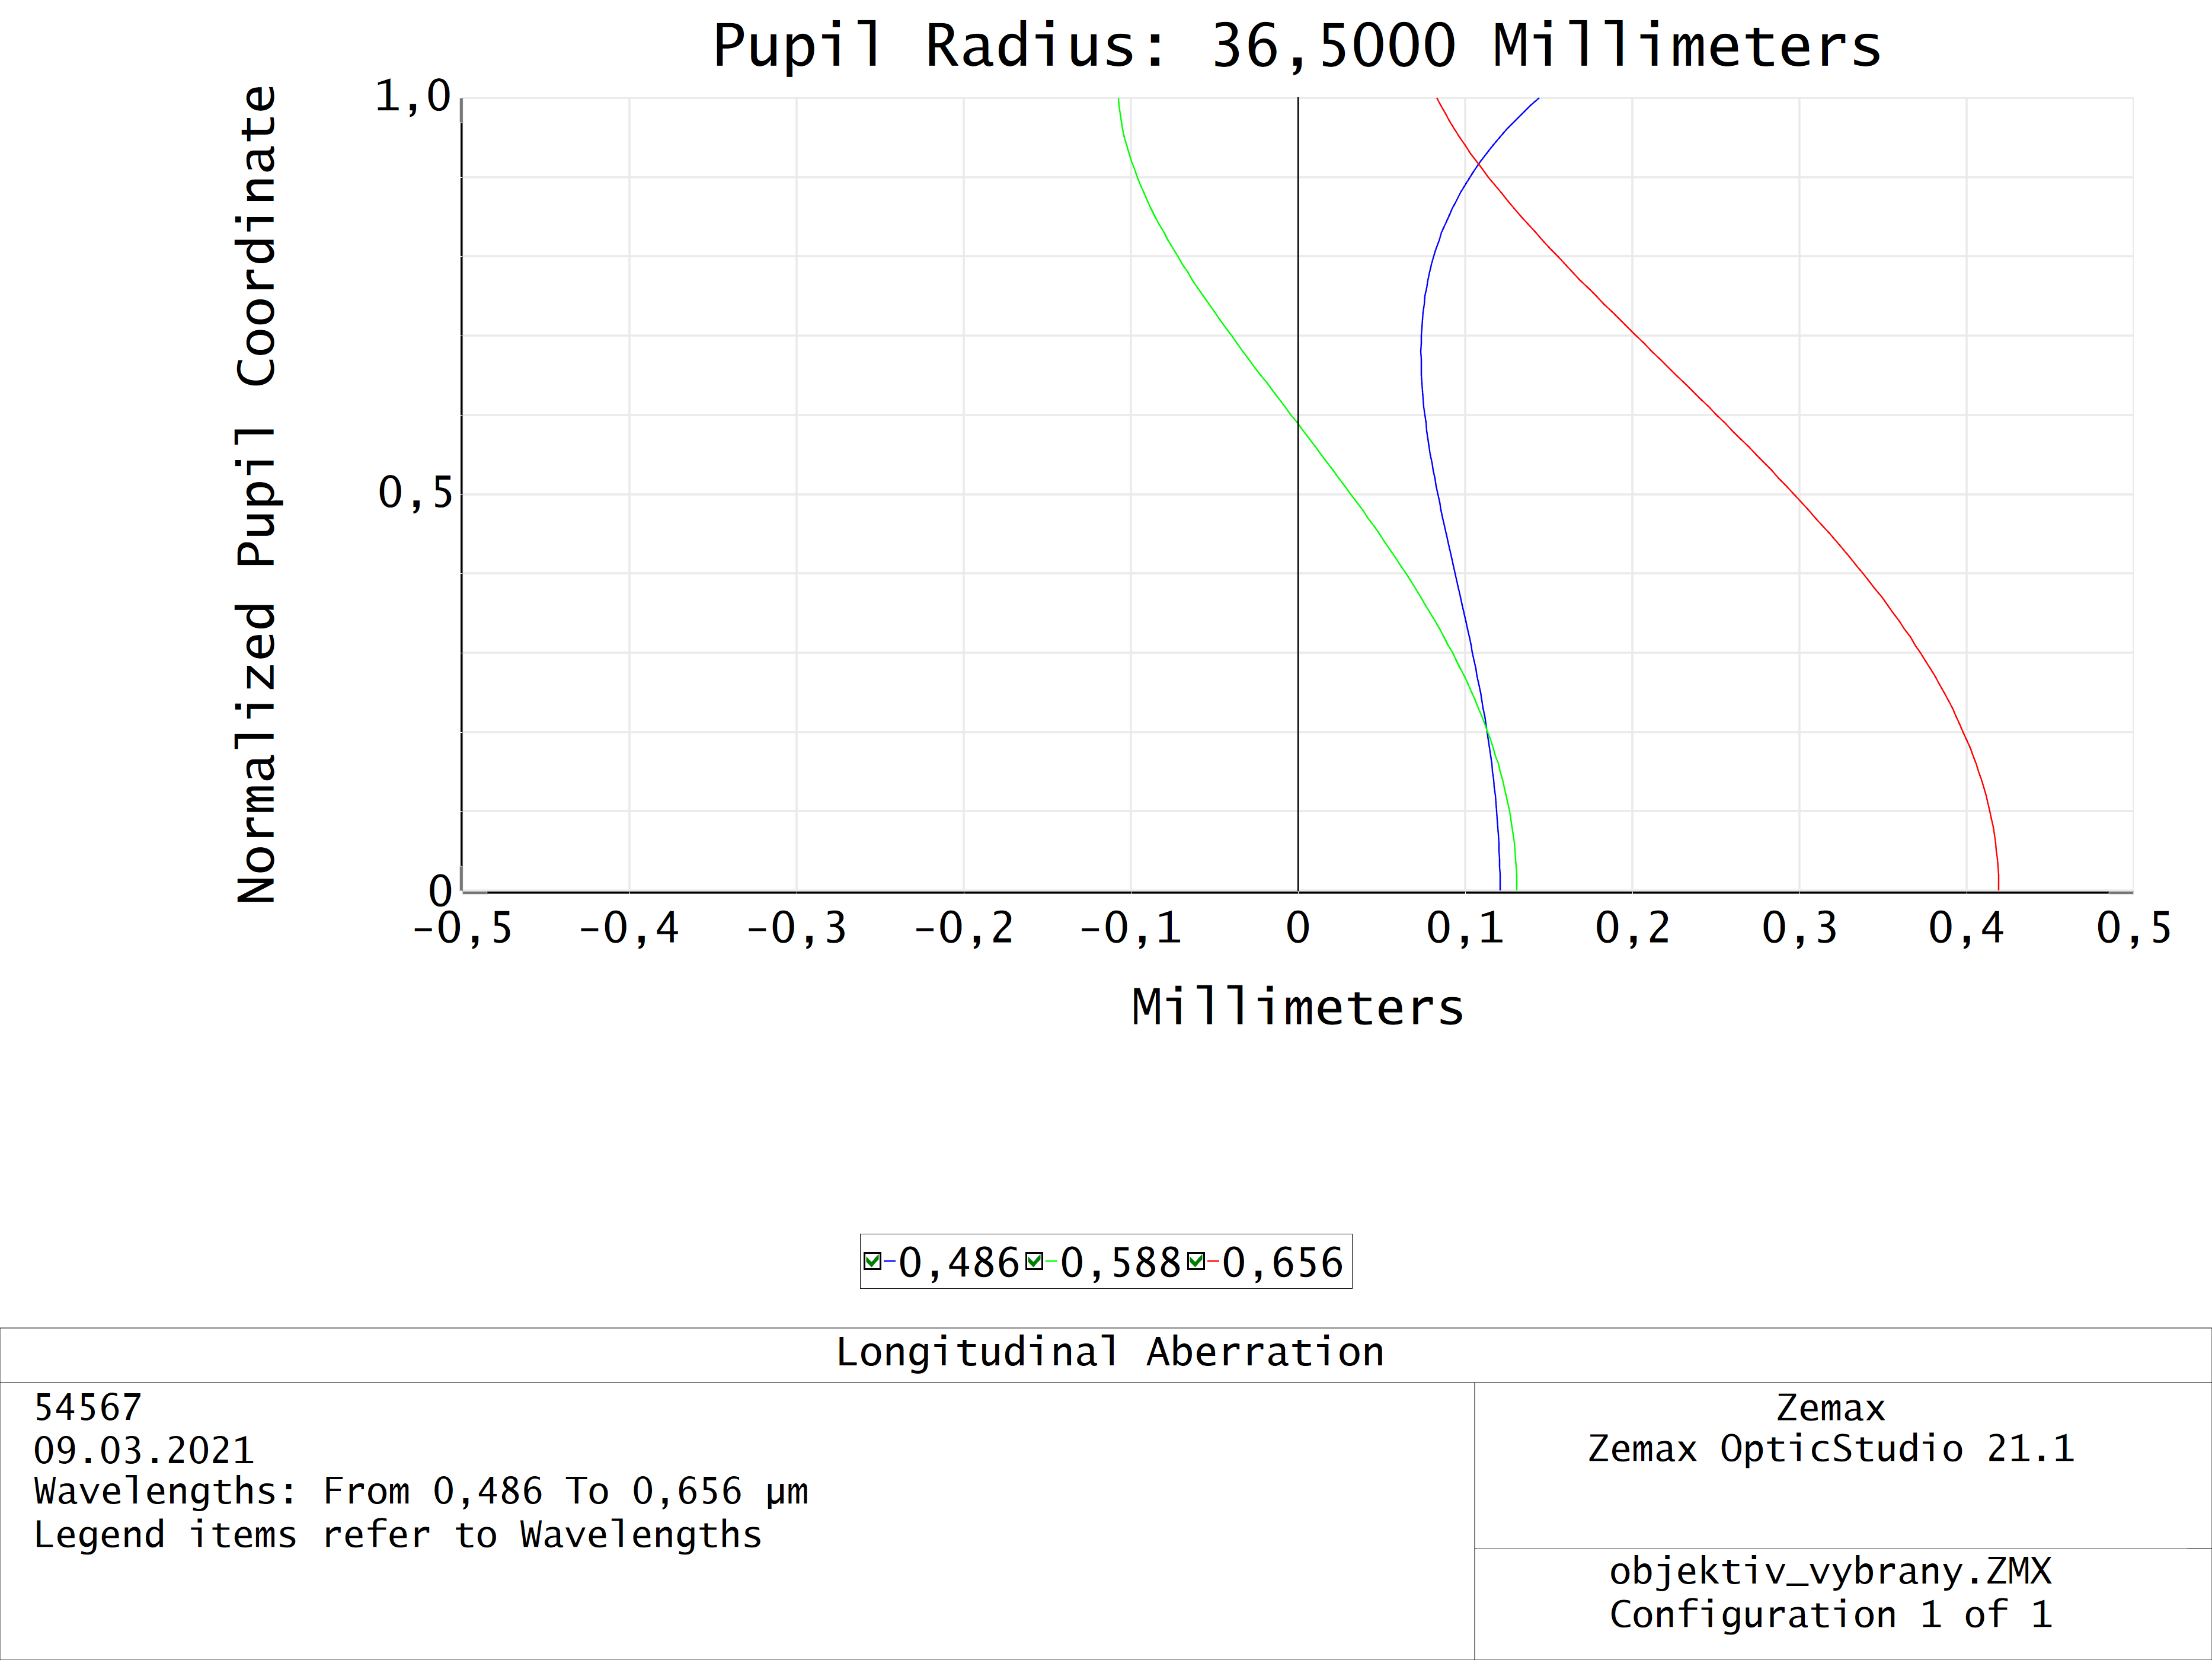
\includegraphics{imgs/LongitudinalAberration_dudlet.png}
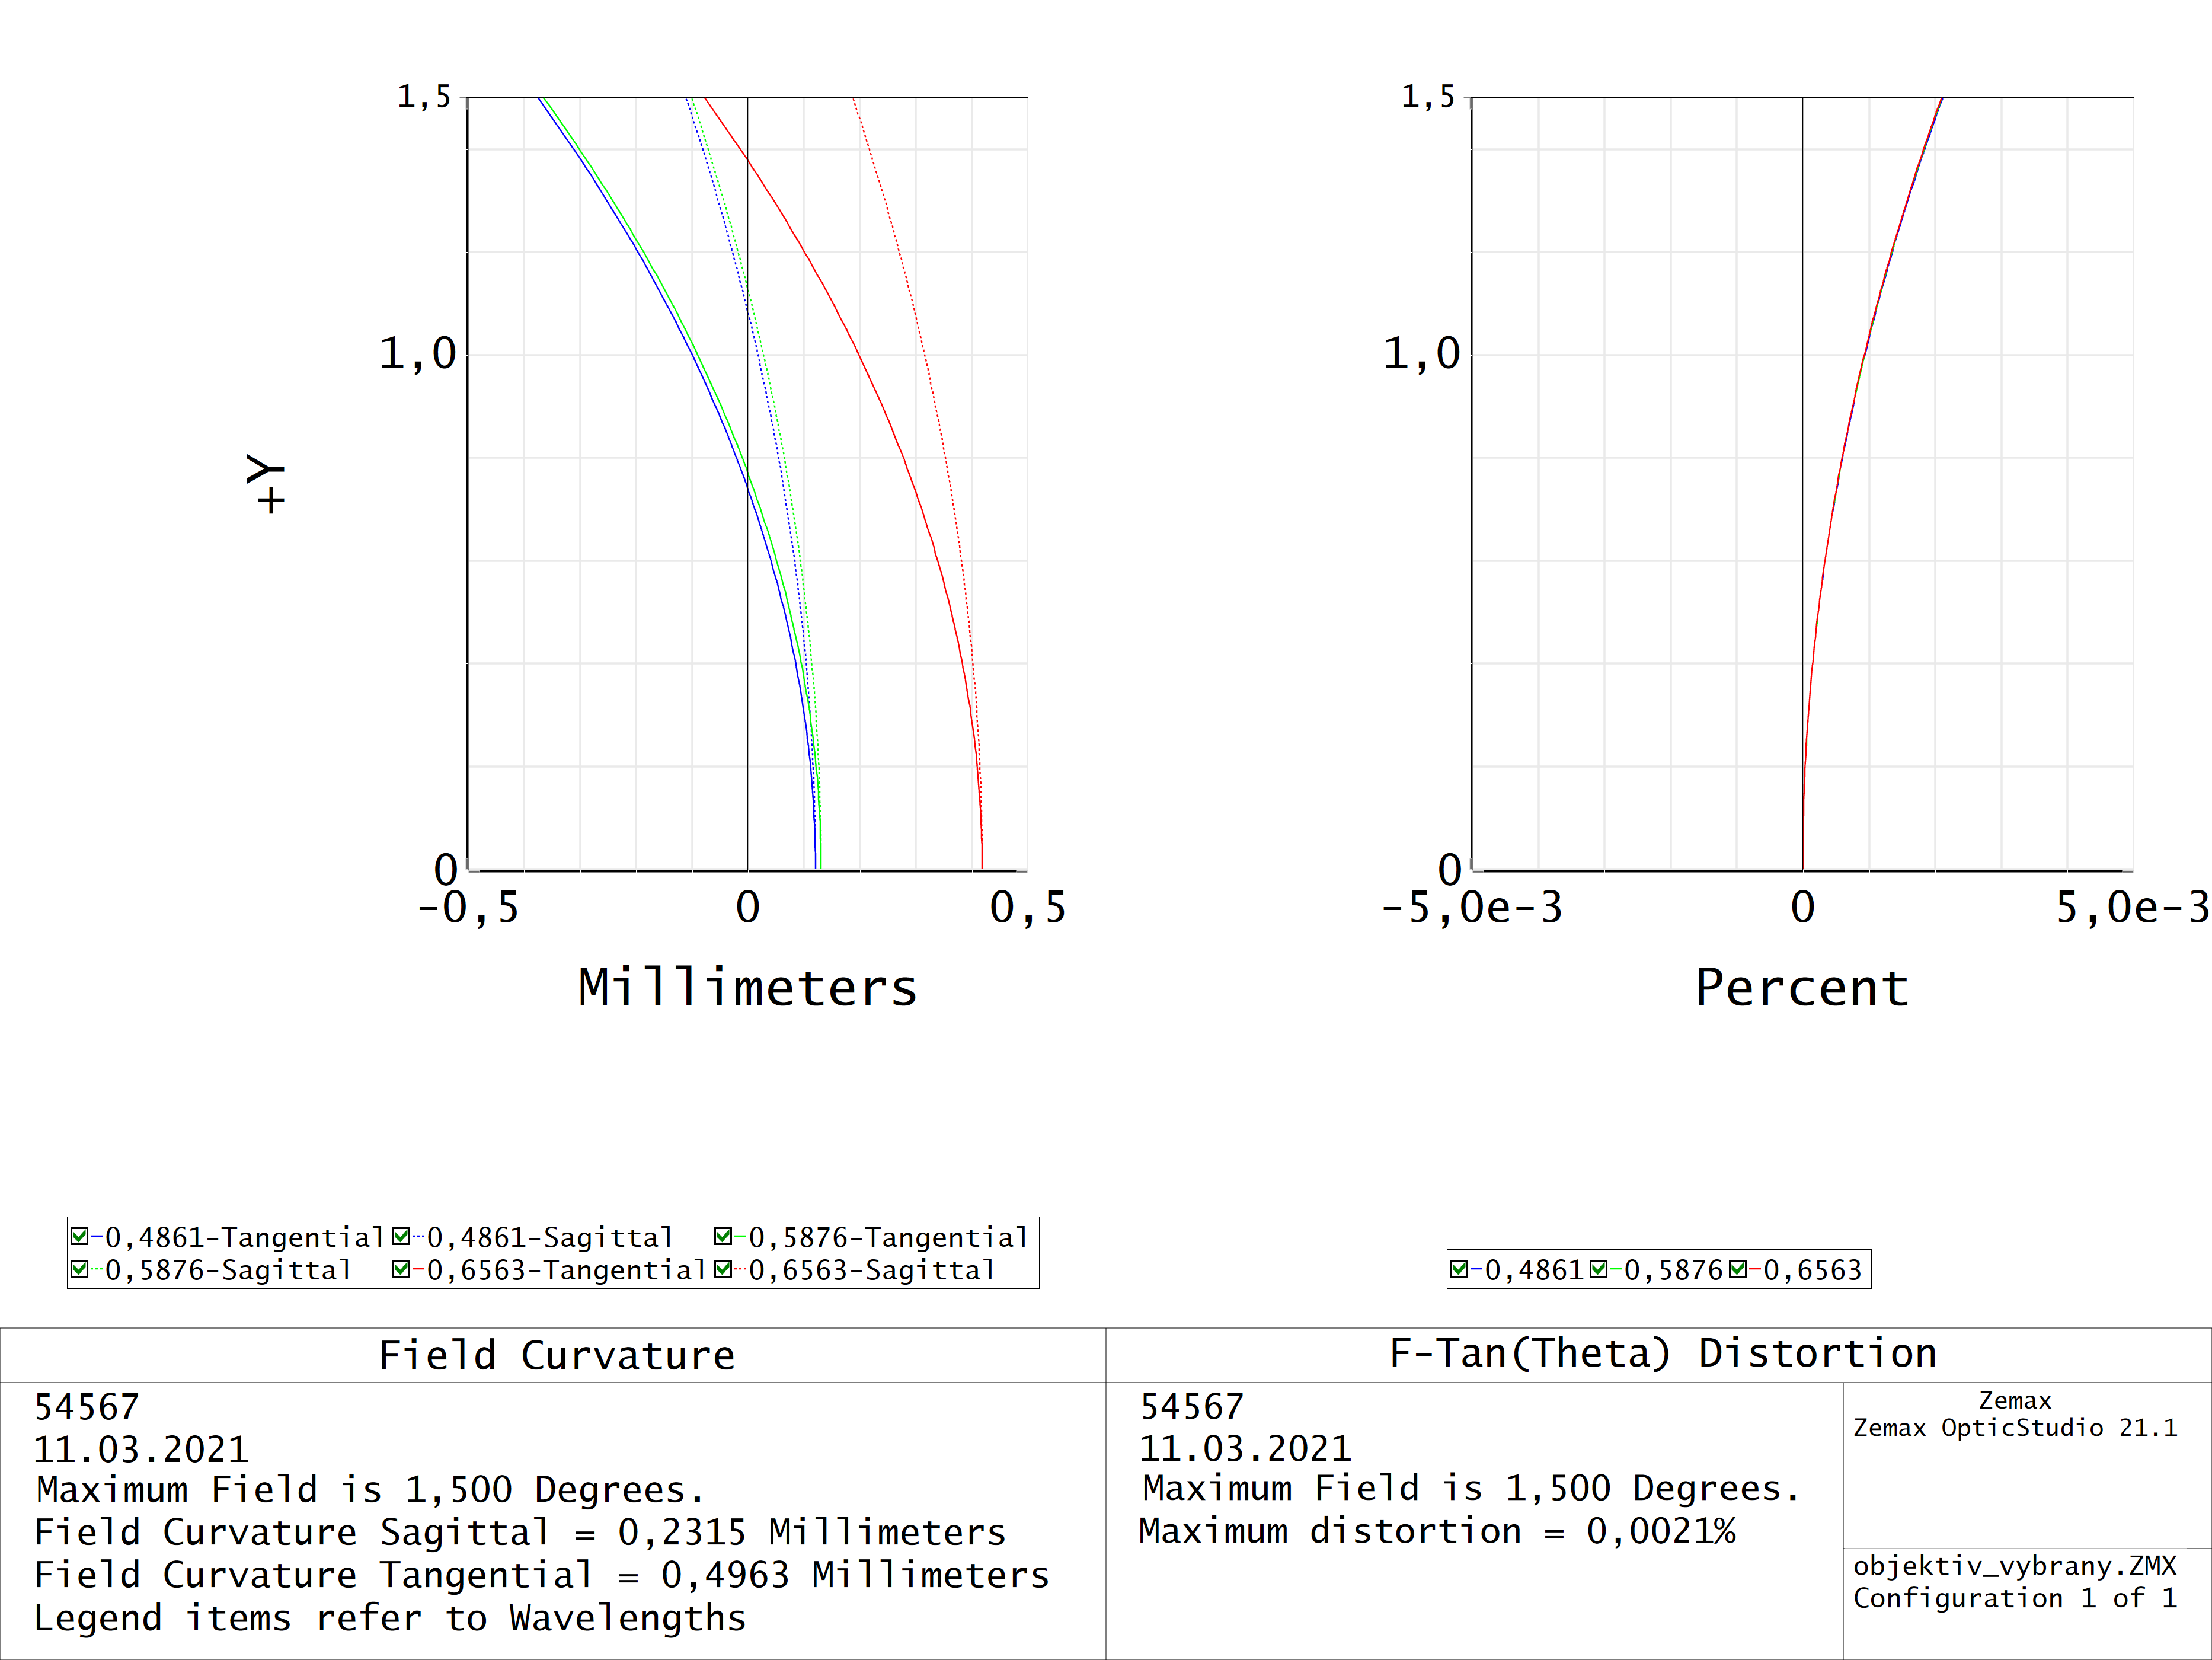
\includegraphics{imgs/FieldCurvDist_dublet.png}

Pro převrácení obrazu bylo jako převracecí mechanizmus vybráno zenitové
zrcátko. Okulár má ohniskovou vzdálenost 16,2 až 5,55 mm a pro použitý
objektiv s ohninskem 400 mm získáváme zorné pole od 1,48° do 0,74°
(velikost předmětu v polní rovnině od 5,17 mm do 2,584 mm). Při návrhu
mechanické části je počítáno, že ohnisková rovina se nachází v rovině
vstupní pupily. Schéma lze vidět na následujícím obrázku.

\begin{figure}
\centering
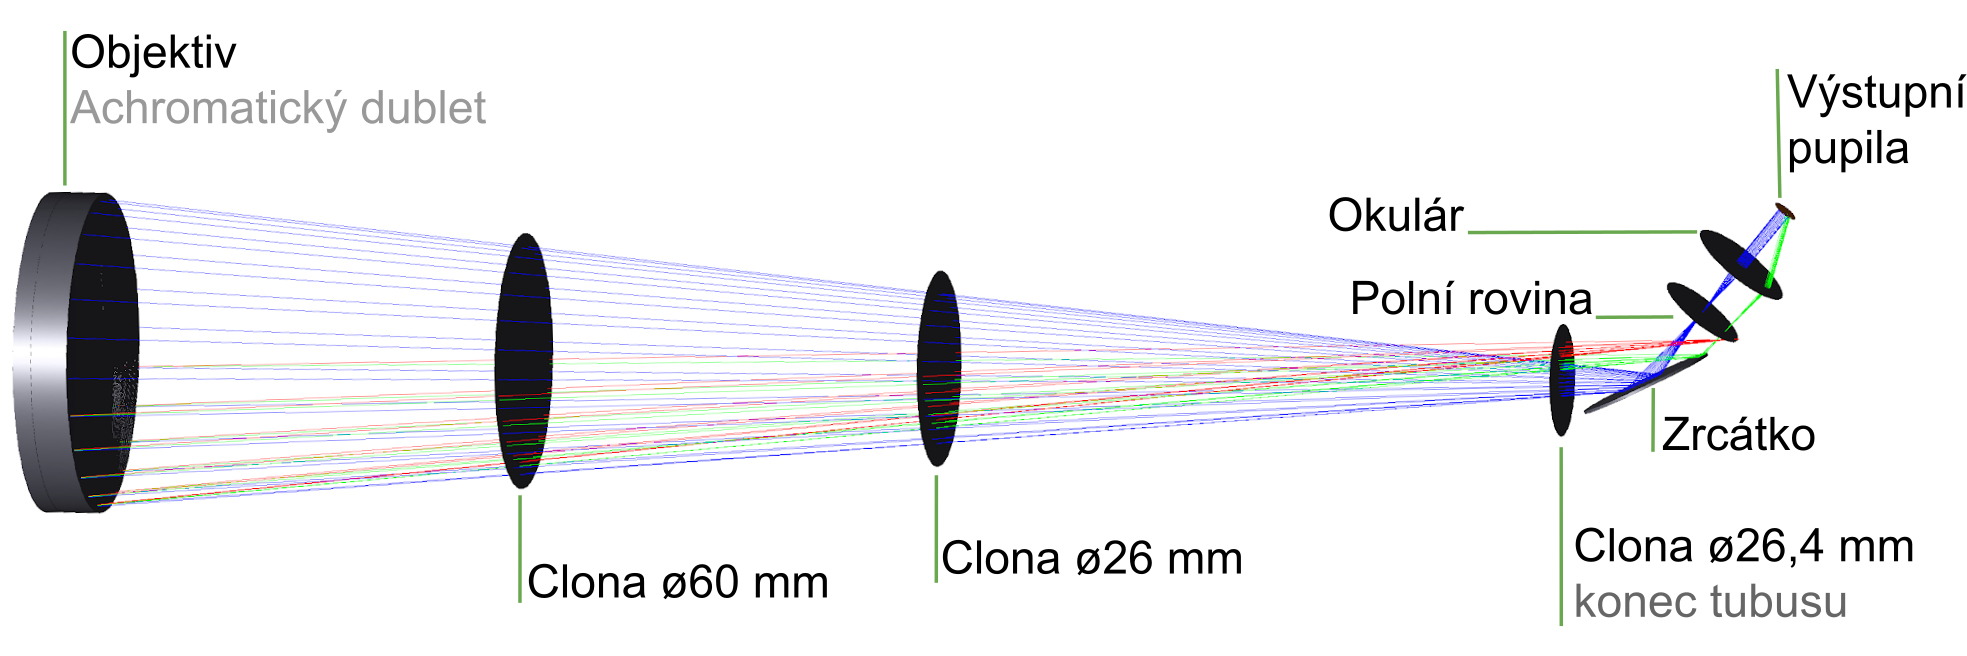
\includegraphics{imgs/schema.png}
\caption{Schéma dalekohledu}
\end{figure}

Poloha okuláru je volena tak, aby okulár zobrazoval polní rovinu do
konvenční zrakové vzdálenosti 250 mm. Při použití delšího ohniska
okuláru (16,2 mm) vzniknou v této rovně stopy velké zhruba 300 μm.
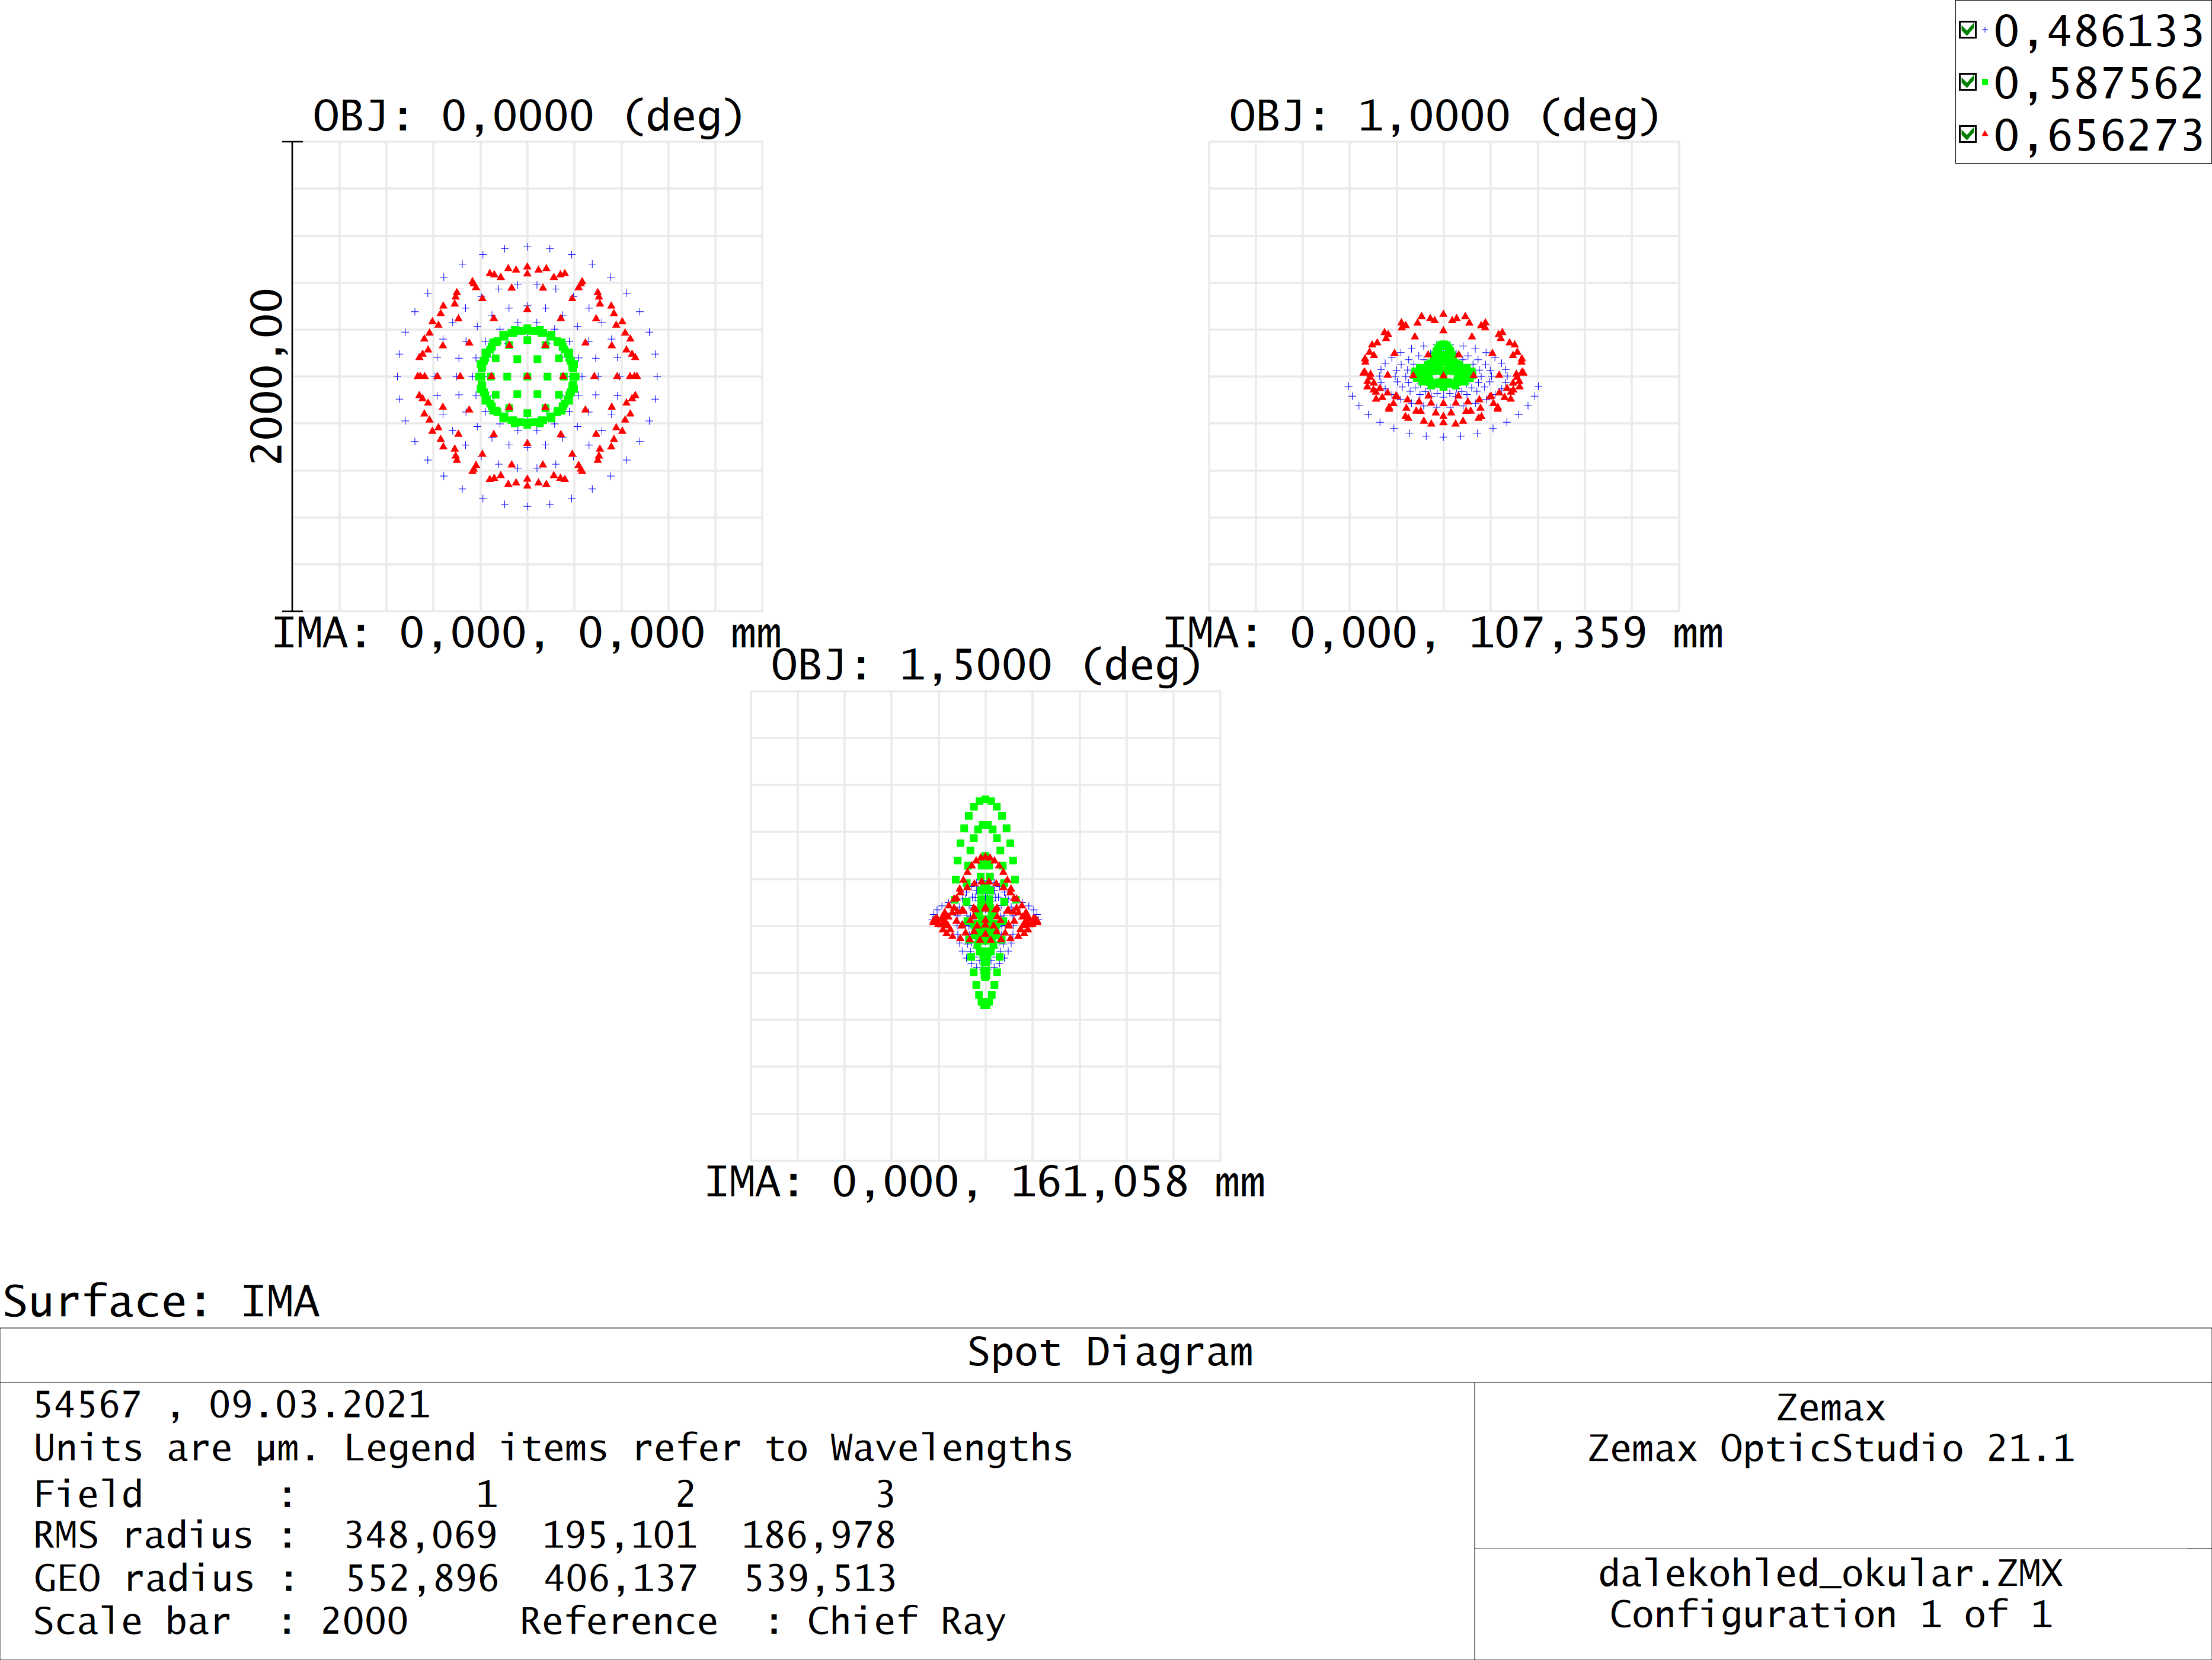
\includegraphics{imgs/SpotDiagram_oko_16mm.png}

Funkce přenosu kontrastu bude vypadat následujícně.

\begin{figure}
\centering
\includegraphics{imgs/FFTMTF.png}
\caption{MTF 16 mm}
\end{figure}

Při použití nejkratšího ohniska okuláru 5,17 mm se vlivem vinětace omezí
zorné pole na zhruba 0,4°.

\begin{figure}
\centering
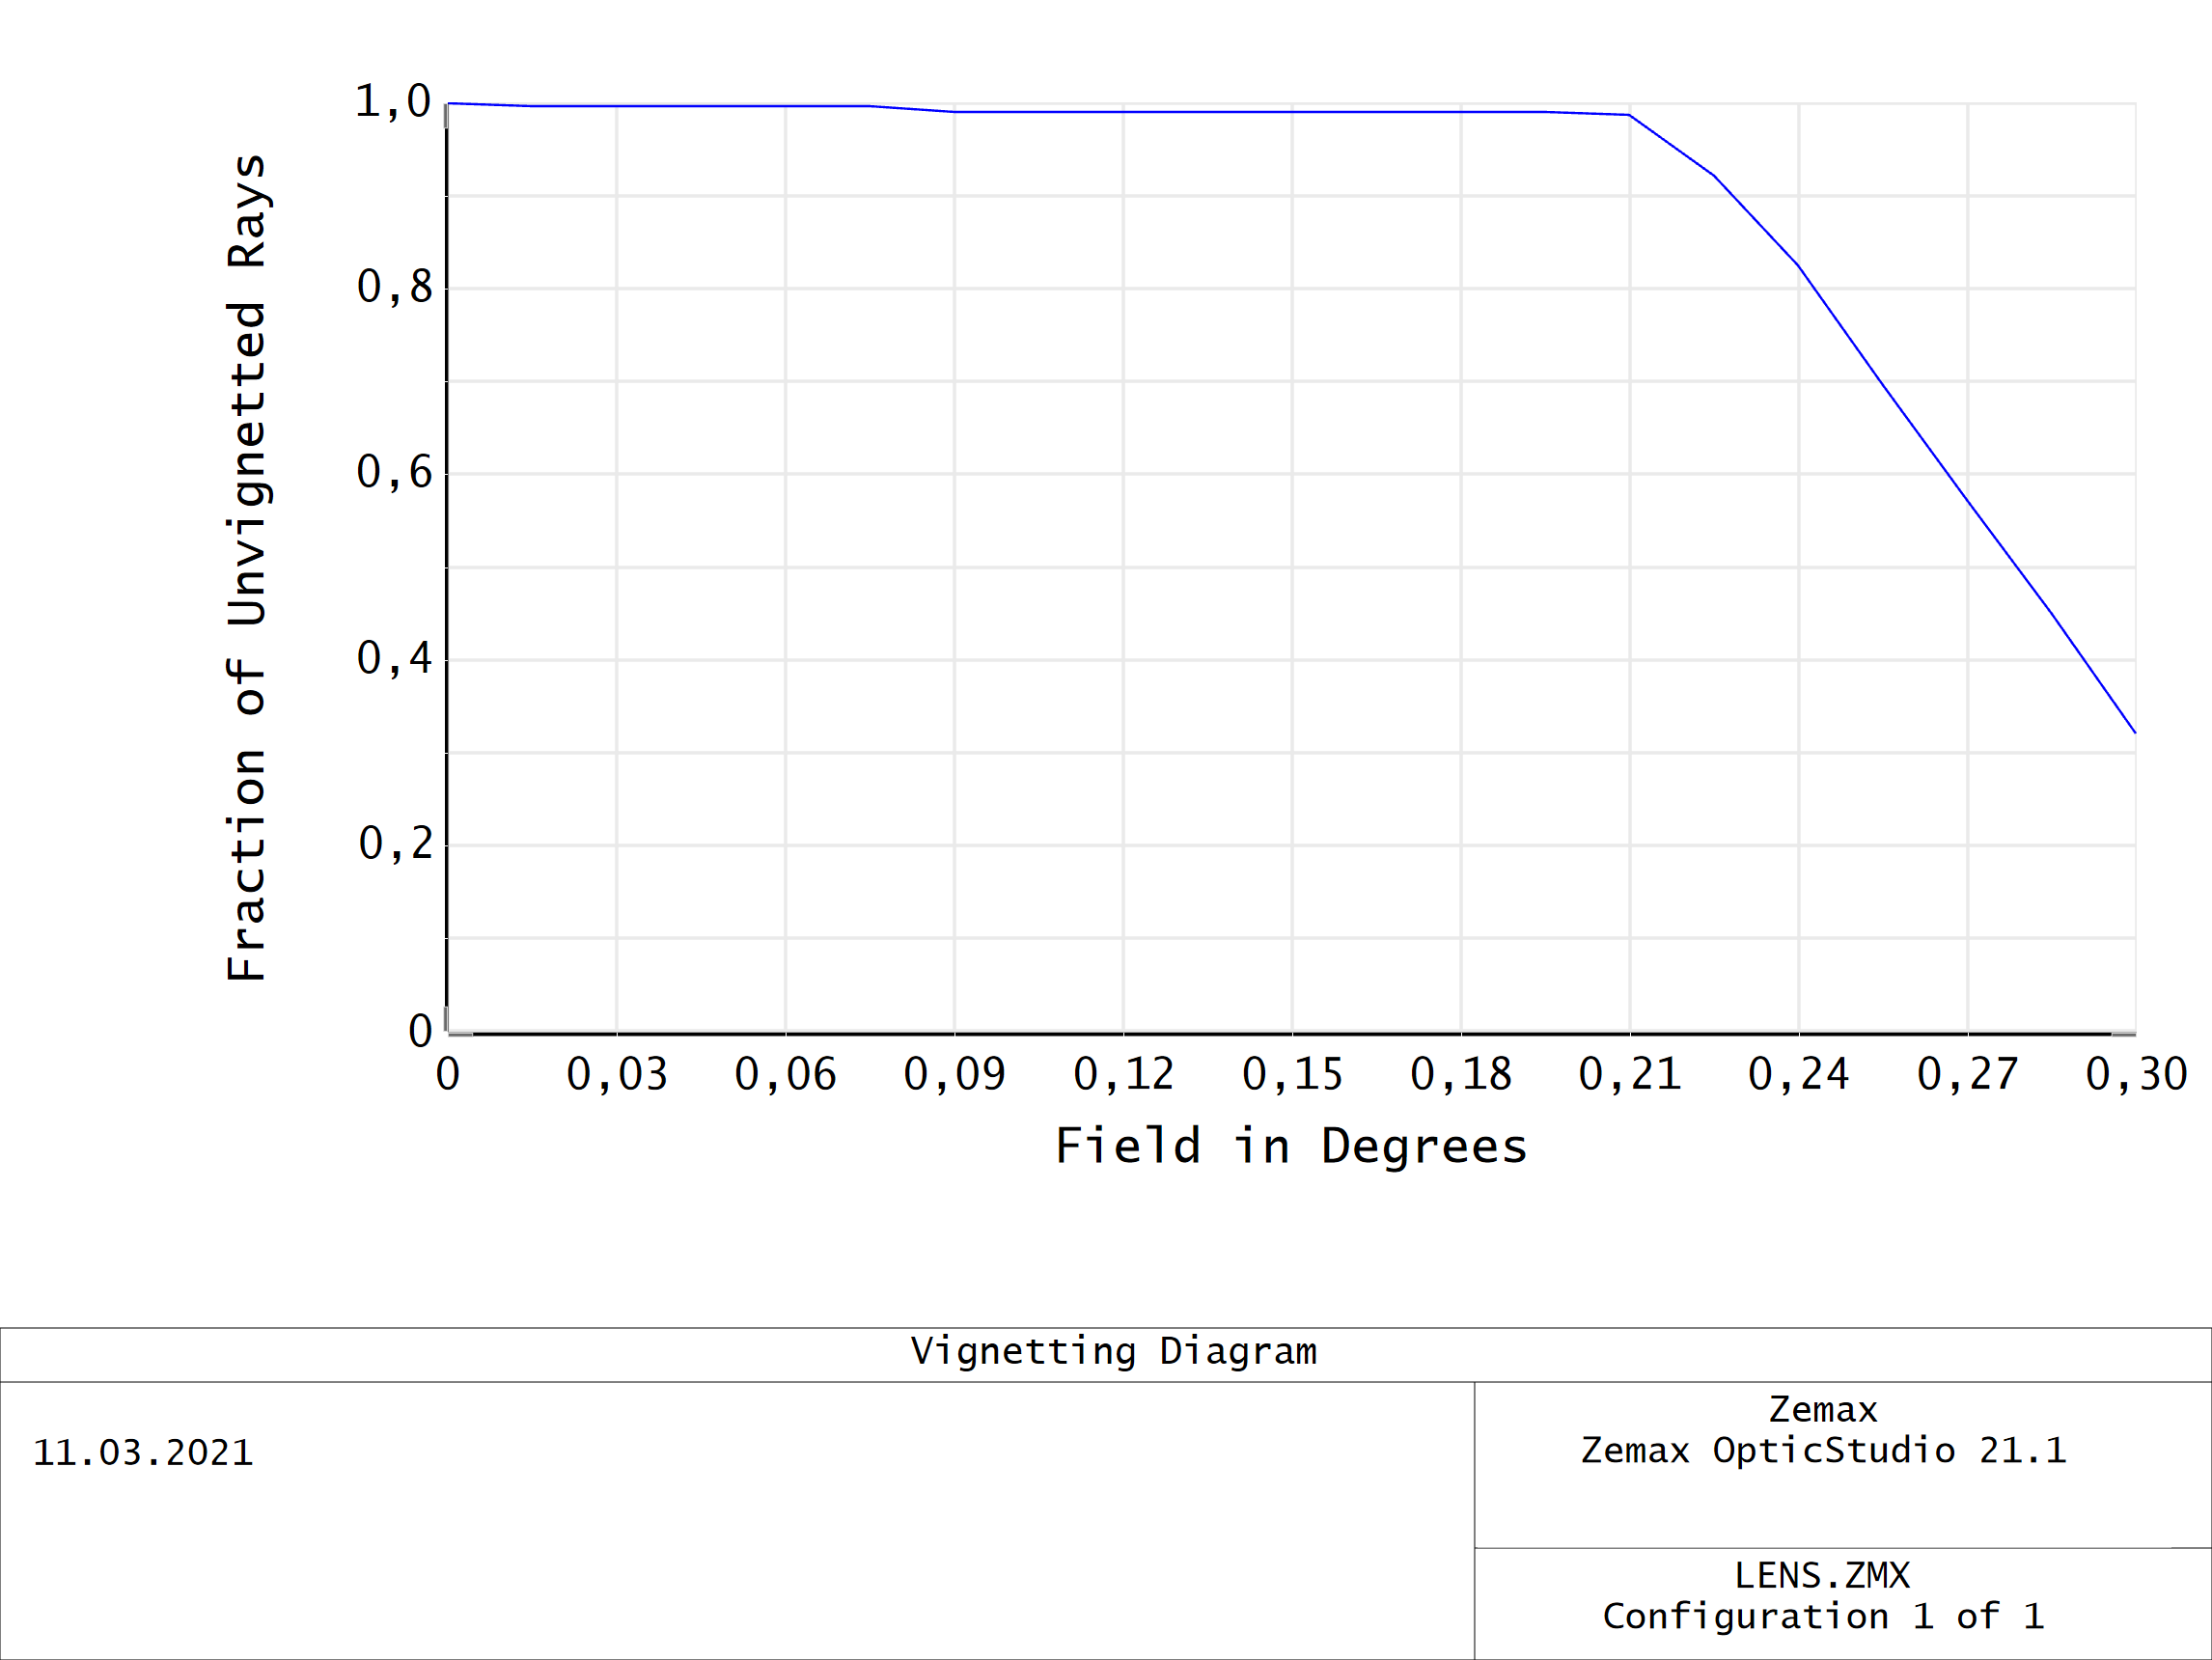
\includegraphics{imgs/VignettingDiagram_5mm.png}
\caption{Vinětace systému}
\end{figure}

V této rovině vznikají stopy velké zhruba 300 μm.

\hypertarget{vuxfdpoux10det-ostux159uxedcuxedho-rozsahu}{%
\subsubsection{Výpočet ostřícího
rozsahu}\label{vuxfdpoux10det-ostux159uxedcuxedho-rozsahu}}

Z rovnice paraxiální čočky lze vypočítat rozsah výsuvu potřebný pro
ostření mězi nekonečněm a předmětem umístěným ve vzdálenosti 20 m. Pro
předmět umístěný v 20 metrech vychází obrazová vzdálenost a' = f' +
8,141 mm. Dále je zapotřebí započítat korekci vad oka v rozsahu 4D.
Užitím vztahu ze strany 19 {[}\protect\hyperlink{lit}{1}{]} zjistíme, že
při použití delšího ohniska 16,2 mm vyžaduje korekce vady přidání
dalších 0,4 mm k výsuvu a to na obě strany.

\begin{longtable}[]{@{}rrr@{}}
\toprule
\begin{minipage}[b]{0.33\columnwidth}\raggedleft
předmnětová vzdálenost\strut
\end{minipage} & \begin{minipage}[b]{0.43\columnwidth}\raggedleft
vzdálenost obrazu od ohniska\strut
\end{minipage} & \begin{minipage}[b]{0.15\columnwidth}\raggedleft
vzdálenost s korekcí pro 4D\strut
\end{minipage}\tabularnewline
\midrule
\endhead
\begin{minipage}[t]{0.33\columnwidth}\raggedleft
inf\strut
\end{minipage} & \begin{minipage}[t]{0.43\columnwidth}\raggedleft
0 mm\strut
\end{minipage} & \begin{minipage}[t]{0.15\columnwidth}\raggedleft
- 0,400 mm\strut
\end{minipage}\tabularnewline
\begin{minipage}[t]{0.33\columnwidth}\raggedleft
20 m\strut
\end{minipage} & \begin{minipage}[t]{0.43\columnwidth}\raggedleft
8,141 mm\strut
\end{minipage} & \begin{minipage}[t]{0.15\columnwidth}\raggedleft
8,541 mm\strut
\end{minipage}\tabularnewline
\bottomrule
\end{longtable}

\begin{figure}
\centering
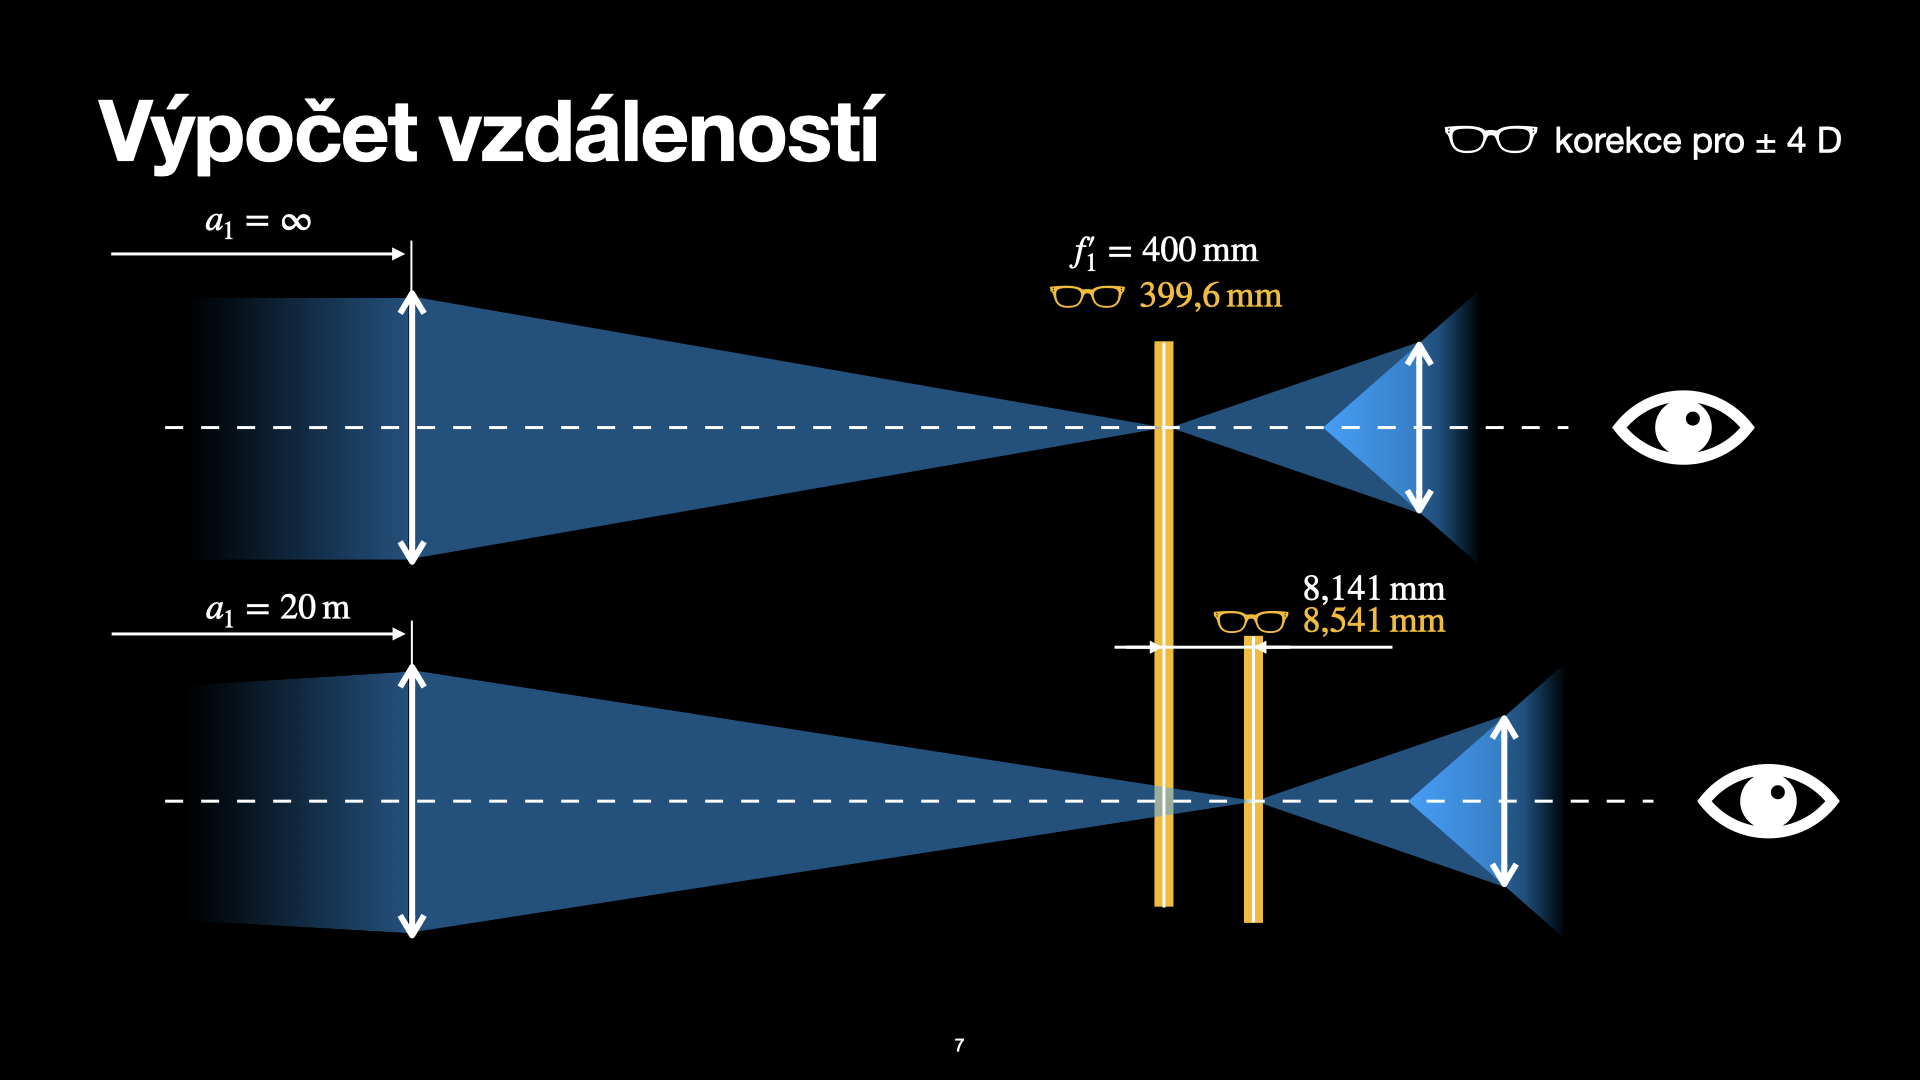
\includegraphics{imgs/rozsah.png}
\caption{Ostřící rozsah}
\end{figure}

Při tvorbě mechanického návrhu je dále počítáno s 0,5 mm rezervou, tak
aby šlo přeostřit ``za nekonečno'' i před 20 m.

\hypertarget{nuxe1vrh-mechanickuxe9-konstrukce}{%
\subsection{Návrh mechanické
konstrukce}\label{nuxe1vrh-mechanickuxe9-konstrukce}}

Pro mechanickou konstrukci jsem volil rozvržení jak lze vidět na obrázku
níže. Pro podrobnější vhled doporučuji nahlédnout do
\href{CAD/drawings/TKC_000.pdf}{výkresu sestav}.

\begin{figure}
\centering

\includegraphics{imgs/dalekohledy_1.png}
\caption{Dalekohledy}
\end{figure}

Objektiv je uložen v objímce, která je závitem připojená k tubusu.
Detail uložení lze vidět na následujícím obrázku.

\begin{figure}
\centering
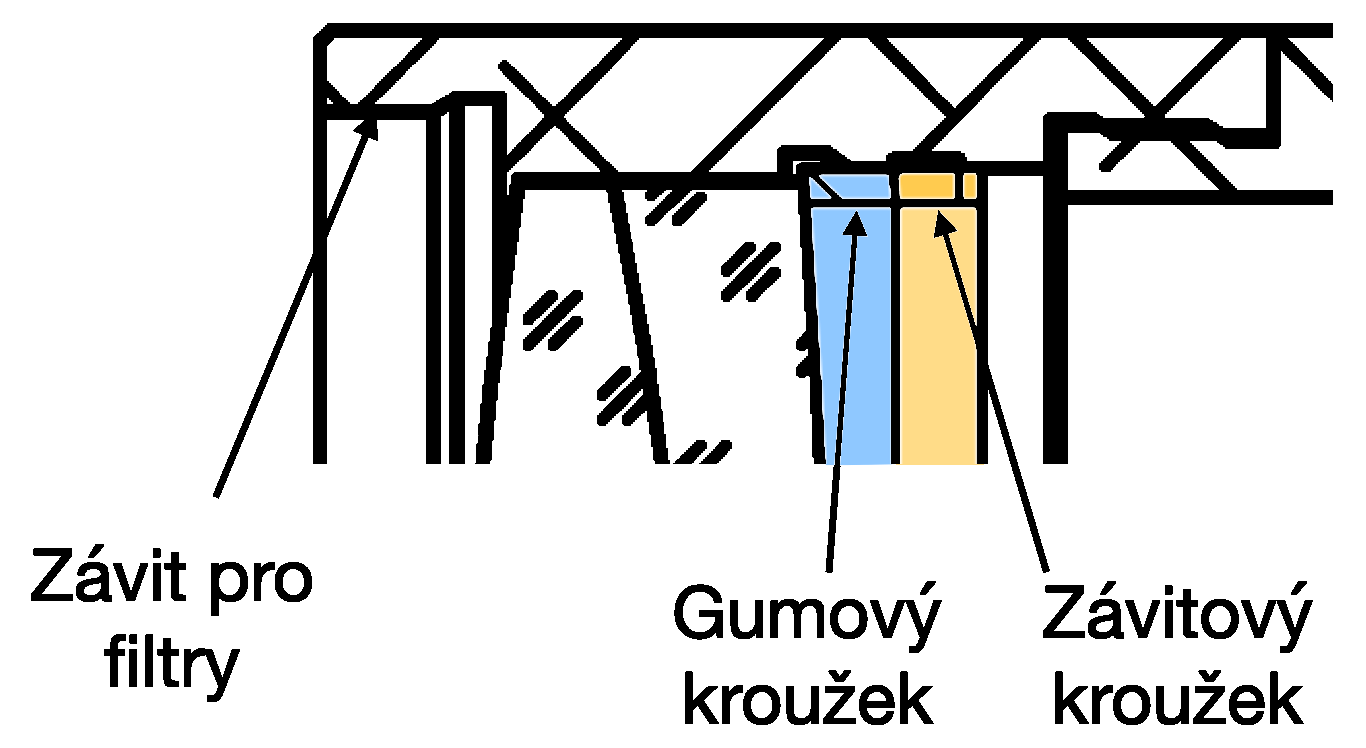
\includegraphics{imgs/ulozeni_objektivu.png}
\caption{Uložení objektivu}
\end{figure}

Tubus je nevržený tak, aby tvarem ušetřil materiál a byl zároveň co
nejrobustnější. Bohužel však tato konstrukce je obrížně vyrobitelná.
Proto pro případ výroby je vhodné vytvořit tubus podle následujícího
schématu.

\begin{figure}
\centering
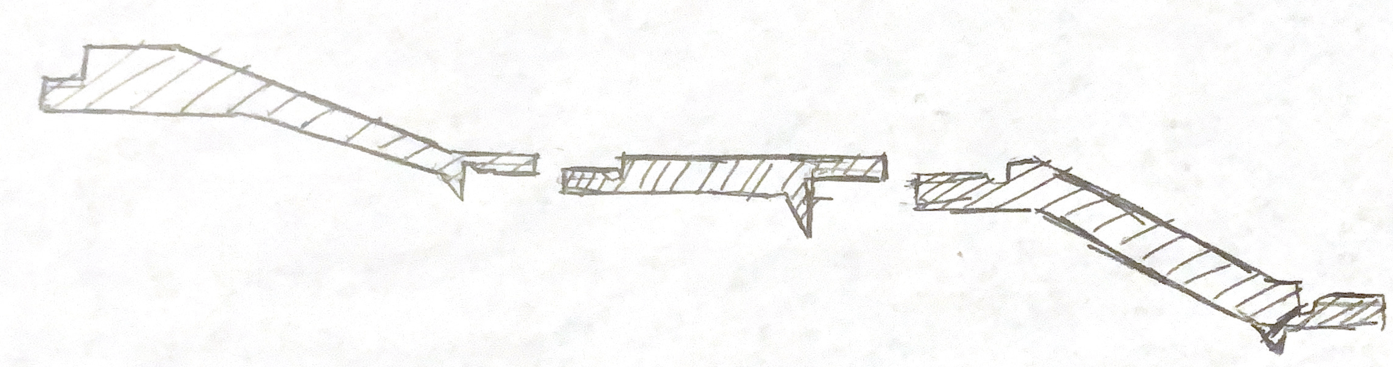
\includegraphics{imgs/vylepseny_tubus.png}
\caption{Upravený tubus}
\end{figure}

Každá z částí by byla zhruba 10 cm dlouhá, proto by byla snáze
vyrobitelná. Jednotlivé části by byly spojeny závitem a na prostřední
rovné části by byla uplá přípojka na stativ, přičmž by pro režim
fotografování snadno šlo vyvažovat soustavu.

Uvnitř kostky připojené k tubusu se nachází
\href{https://www.edmundoptics.com/p/elliptical-mirror-2223mm-minor-axis-protected-aluminum/1919/}{eliptické
zrcátko} od firmy Edmund Optics. Pro obsažení celého pole je zapotřebí
zrcátko s hlavní poloosou 14 mm a vedlejší poloosou 8 mm, což vybrané
zrcátko pohodlně splňuje.

Zrcátko je upevněno na tříbodém justážním mechanizmu, kdy va šouby s
jemným stoupáním tlačí proti pružinkám. Pružinky jsou zajištěny kolíky a
jako osa rotace slouží kalená kulička. Destička s zrcátkem je přikryta
krytem, aby se dovnitř kostky nedostávaly nečistoty zároveň aby nebyly
odkrety justážní šrouby.

\begin{figure}
\centering
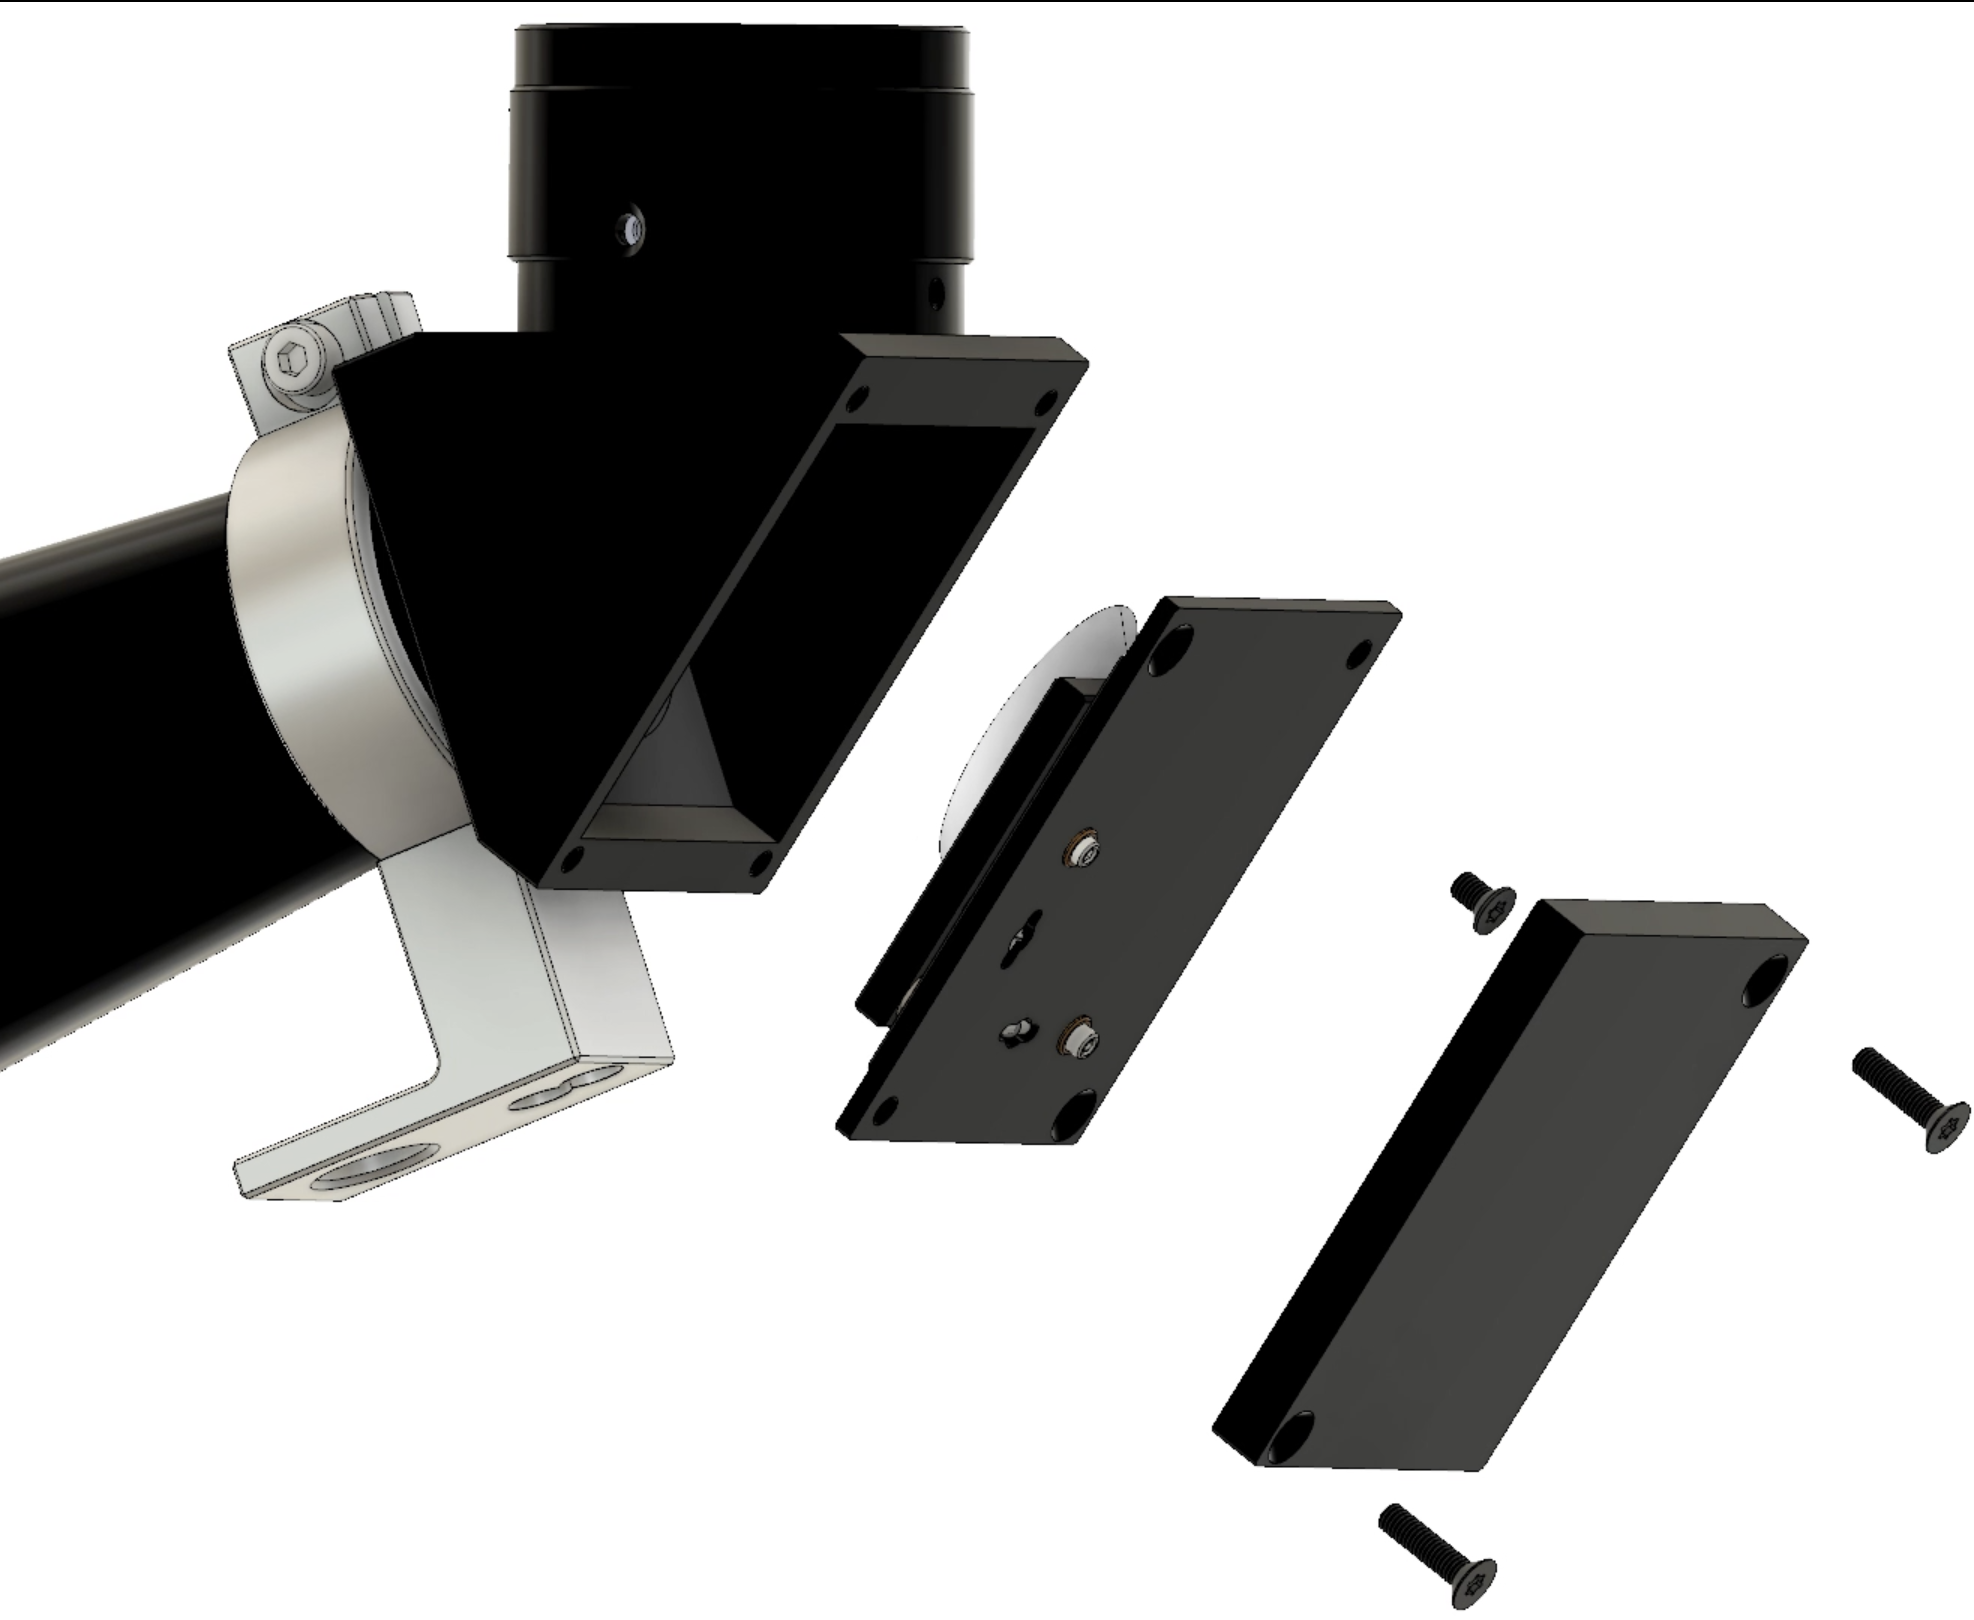
\includegraphics{imgs/justazni_mechanizmus.png}
\caption{Justážní mechanizmus}
\end{figure}

Okulárový výsuv je řešen pomocí závitu. Hmatník je pomocí dvou
C-prstenců připevněn k statickému dílu a pomocí závitu na vnitřní straně
se posouvá vnitřní díl. Ve vnitřním dílu je drážka, která omezuje pohyb
dílu.

\begin{figure}
\centering
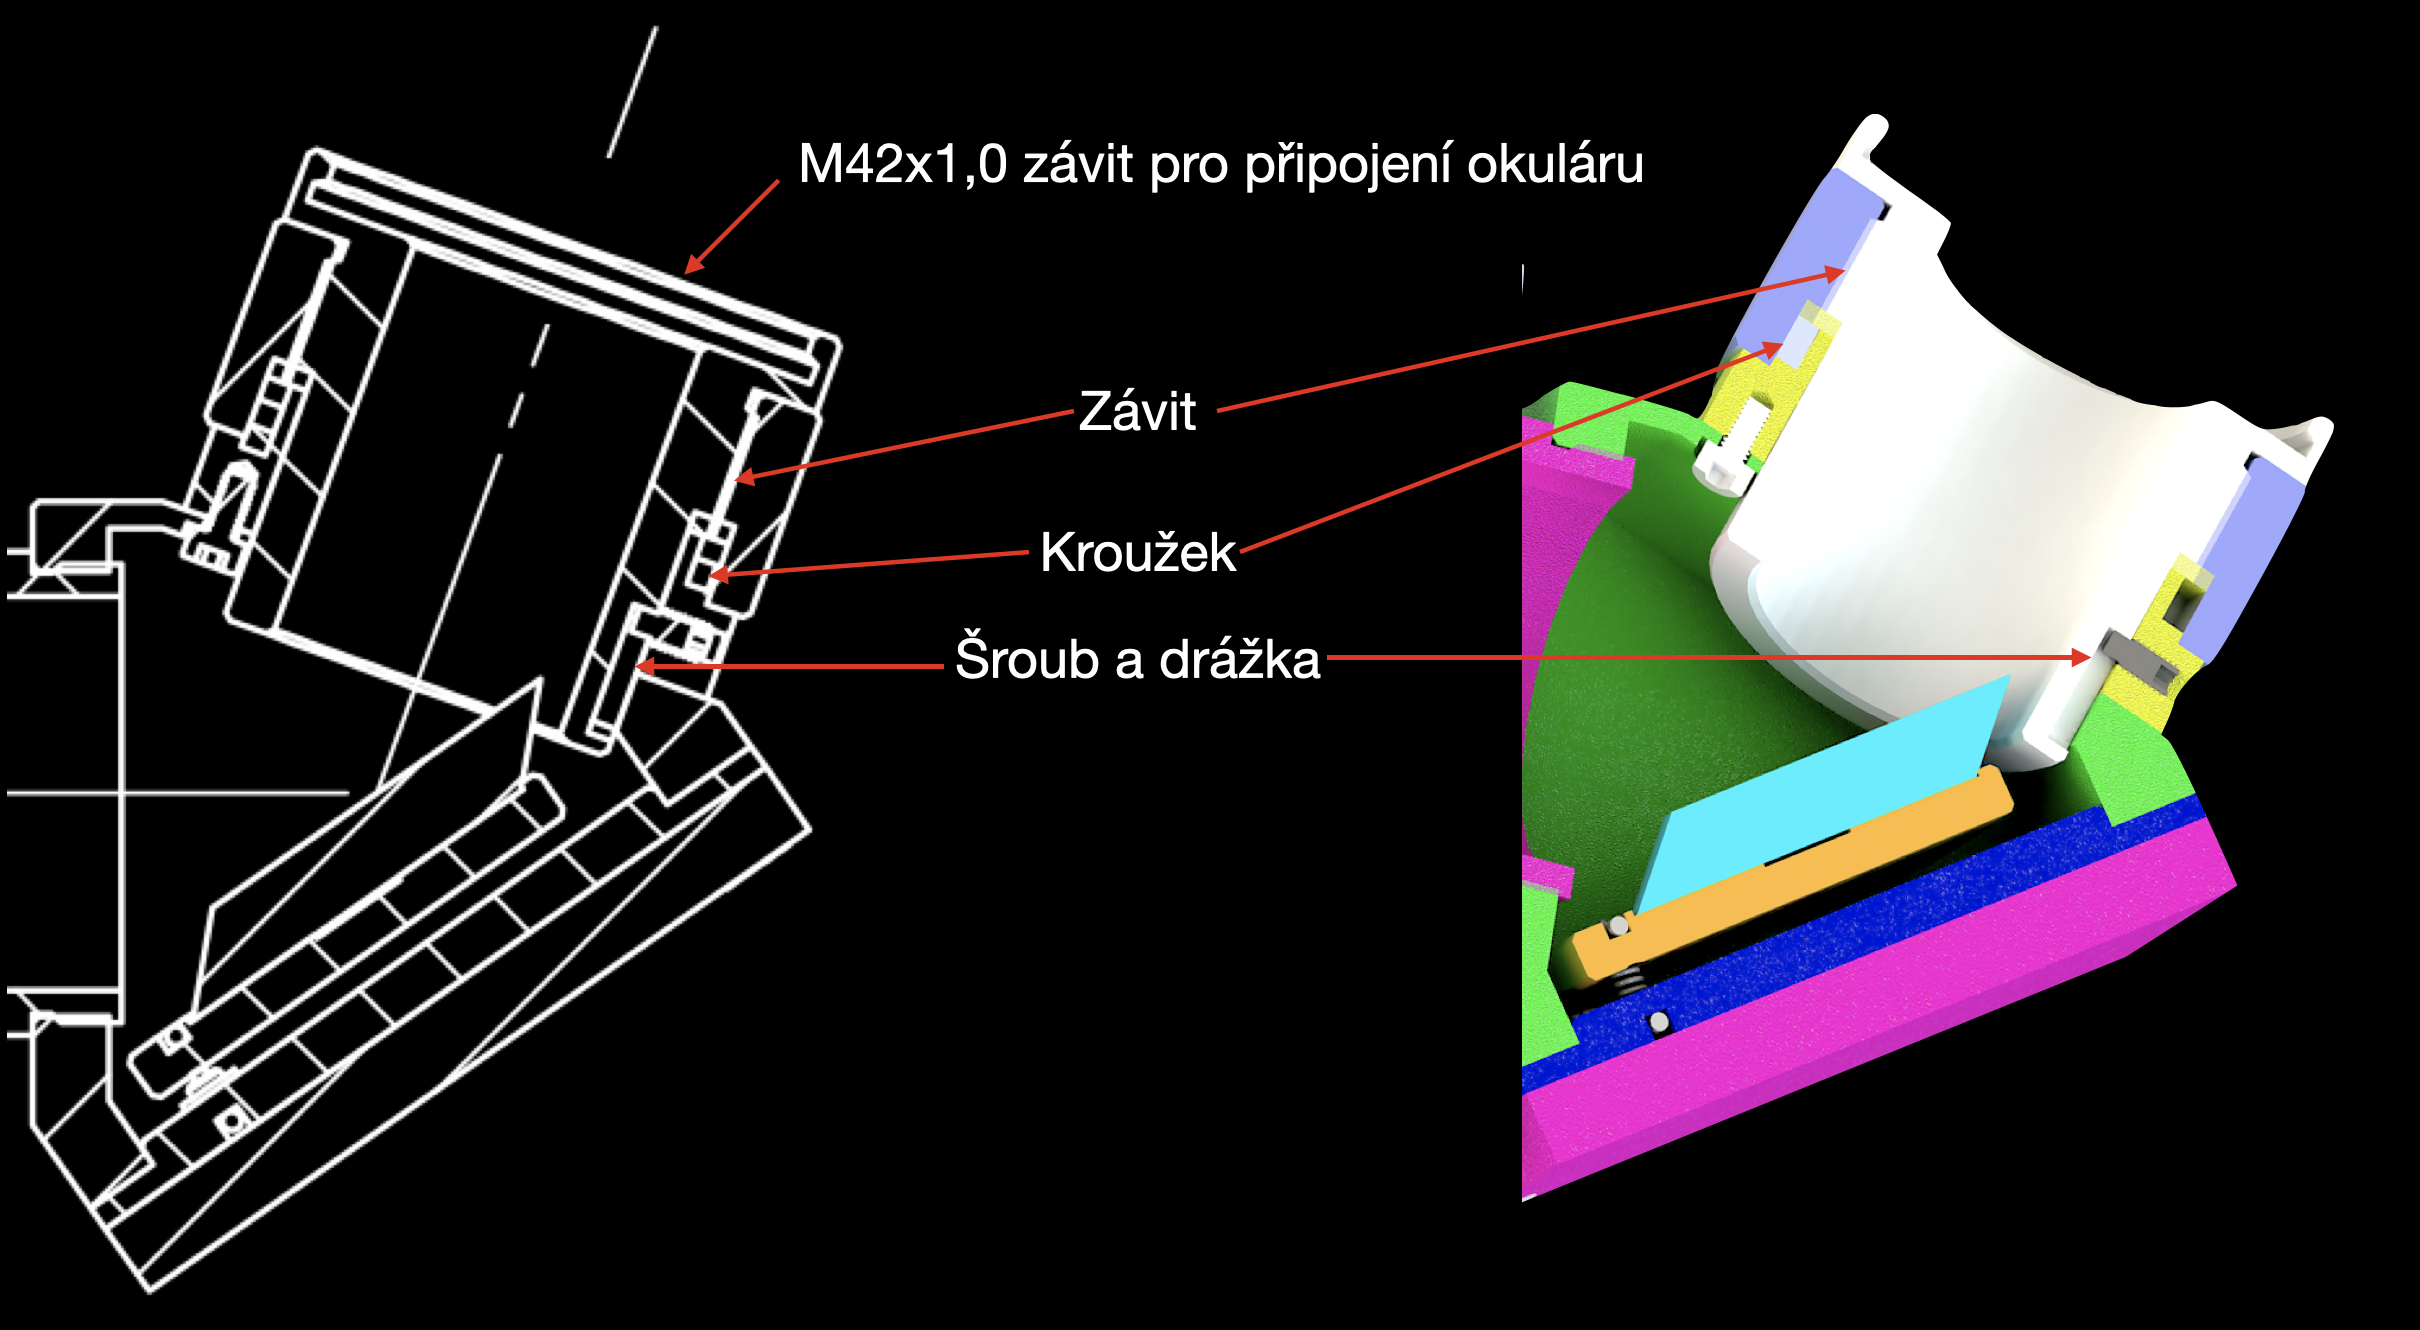
\includegraphics{imgs/vysuv.png}
\caption{Výsuv}
\end{figure}

Při fotografování je zapotřebí odšroubovat kostku se zenitovým zrcátkem
a připojit výsuv zakončený M42 bajonetem. Výsuv je řešen obdobně jako v
případě okuláru.

\begin{figure}
\centering
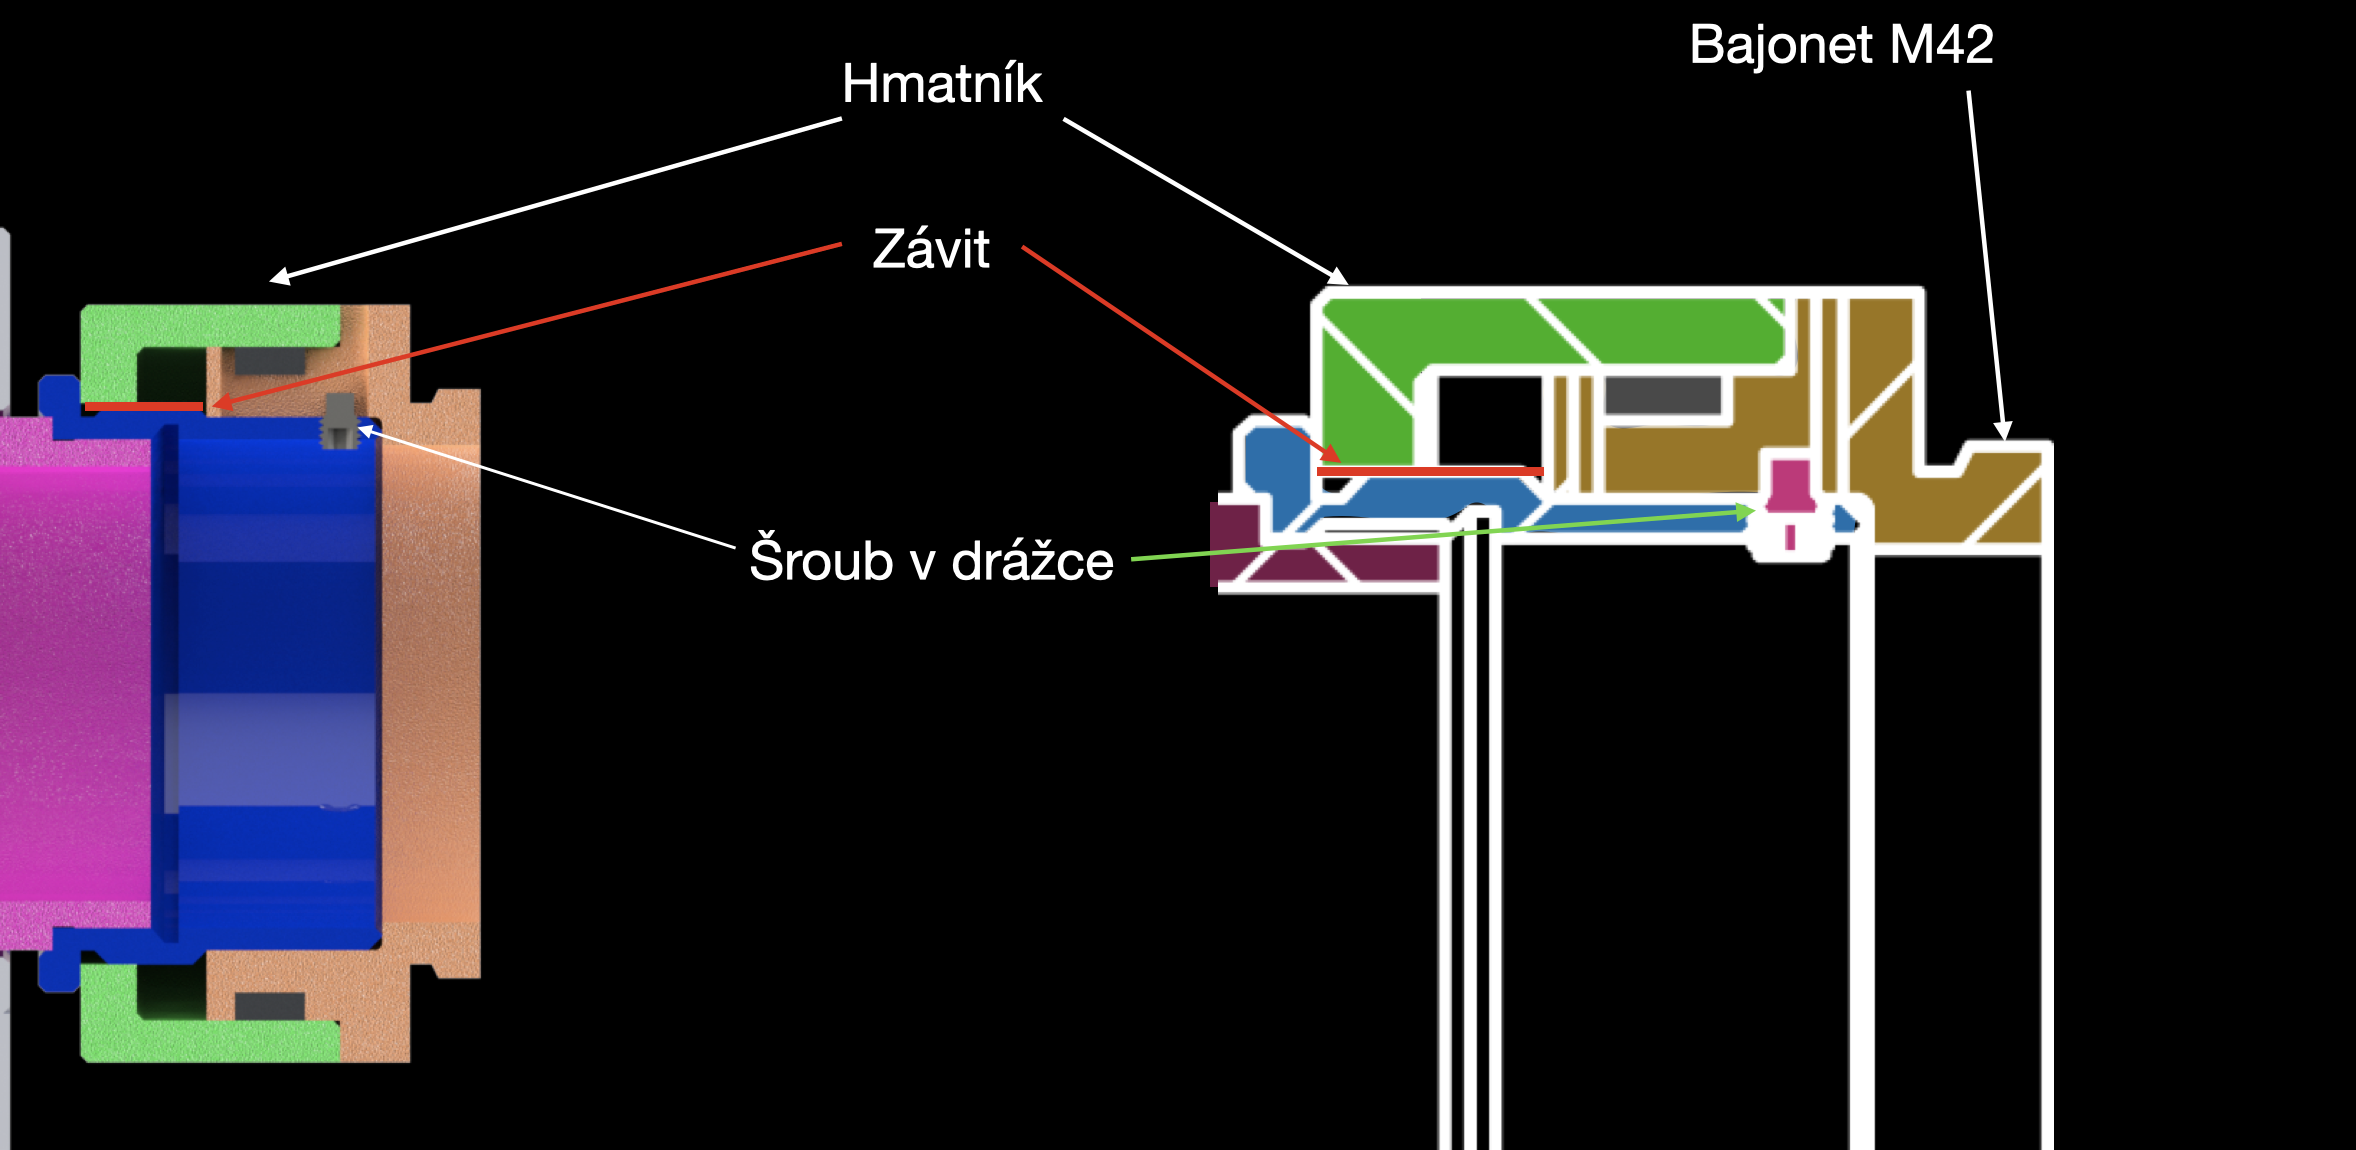
\includegraphics{imgs/vysuv_foto.png}
\caption{Fotografický výsuv}
\end{figure}

\hypertarget{materiuxe1ly-a-dalux161uxed-uxfapravy}{%
\subsubsection{Materiály a další
úpravy}\label{materiuxe1ly-a-dalux161uxed-uxfapravy}}

Jako materiál byla u většiny dílů volena hliníková slitina EN AW 2030
nebo 5083. Díly je zapotřebí po obrábění eloxovat. Pro případné
požadavky přesné výroby vybraných ploch je vhodné nechat před eloxací
drobný přídavek a požadované plochy po eloxaci doobrobit.

\hypertarget{zuxe1vux11br}{%
\subsection{Závěr}\label{zuxe1vux11br}}

Byl úspěšně navržen čočkový dalekohled keplerova typu. Pro dalekohled
byl vybrán vhodný objektiv a okulár. Pomocí počítačové simulace byly
zjištěny jeho optické vlastnosti. Následně bylo vypočítán rozsah výsuvu
potřebný pro pozorování objektů mezi nekonečnem a 20m. Byl vypočítán
rozsah potřebný pro korekci zrakových vad do 4 D. Následně byla navržena
mechanická konstrukce dalekohledu. Pro potřeby výroby byly vytvořeny
výrobní výkresy vybraných dílů a výkres sestavy.

\hypertarget{literatura}{%
\subsection{\texorpdfstring{Literatura
}{Literatura }}\label{literatura}}

{[}1{]} Liška Miroslav: \emph{Optické sešity} {[}cit. 24.5.2021{]} url:
http://physics.fme.vutbr.cz/files/vyuka/OptPristroje/OP7\_Zakladni\%20opticke\%20pristroje.pdf

{[}2{]} Fuka Josef, Havelka Bedřich: \emph{Optika a atomová fyzika}. SPN
Praha 1961.

{[}3{]} Born Max, Wolf Emil: \emph{Principles of optics}. Seventh
anniversary ed, Cambridge University Press 2019.

\end{document}
